\documentclass{scrartcl}
\usepackage[T1]{fontenc}
\usepackage[utf8]{inputenc}
\usepackage[ngerman]{babel}
\usepackage{lmodern}

% some useful packages
\usepackage{mathtools}
\usepackage{amssymb}
\usepackage{graphicx}
\usepackage{hyperref}
\usepackage{titlesec}

\newcommand{\sectionbreak}{\clearpage}

\usepackage{ifthen}

\newenvironment{requirements}{
	\begin{itemize}
}{
	\end{itemize}
}

\newcommand{\req}[2][]{
	\item[/#2/]\label{#2}\ifthenelse{\equal{#1}{}}{}{ \textbf{#1}}
}


\begin{document}
\setlength{\parindent}{0pt}

\begin{titlepage}
\begin{center}
\begin{minipage}{0.4\textwidth}
	\begin{flushleft} \large
		
\includegraphics[height=40pt]{../assets/kitlogo.pdf}
	\end{flushleft}
\end{minipage}
\begin{minipage}{0.4\textwidth}
	\begin{flushright} \large
		
\includegraphics[height=40pt]{../assets/stlogo-600dpi.pdf}
	\end{flushright}
\end{minipage} \\[2cm]
\end{center}
%Title
\begin{center}
	{\huge \bfseries Croggle}\\[0.1cm]
	{\large  Lernanwendung für Grundschüler}
\end{center}


%Subtitle
\begin{center}
	{\Large Pflichtenheft}\\[0.5cm]
\end{center}
%Authors
\begin{center}
	{Lukas Böhm, Tobias Hornberger, Jonas Mehlhaus, \\ Iris Mehrbrodt, Vincent Schüßler, Lena Winter} \\[1cm]
\end{center}

%Date
\begin{center}
	{\large \today}
\end{center}
	
	\vfill
	
	\begin{center}
	
\includegraphics[width=300pt]{../assets/logo.png}
	\end{center}


\end{titlepage}

\iffalse
\title{Pflichtenheft}
\author{ 
	Lukas Böhm\and 
	Tobias Hornberger\and 
	Jonas Mehlhaus\and 
	Iris Mehrbrodt\and 
	Vincent Schüßler \and 
	Lena Winter
}
\date{\today}

\maketitle
\thispagestyle{empty}

\fi
\pagenumbering{roman}

\clearpage
\pagestyle{empty}
\tableofcontents

\clearpage
\pagestyle{plain}
\pagenumbering{arabic}
\setcounter{page}{1}

\section{Einleitung}

Programmieren ist eine immer wichtiger werdende Fähigkeit, die aufgrund des fortschreitenden Einzugs von Computern jeder Form in den Alltag bereits mit Lesen, Schreiben und Rechnen verglichen oder sogar gleichgesetzt wird.
Es gibt verschiedenste Ansätze, Kinder schon sehr früh an das Programmieren heranzuführen.
Eine häufig vertretene Forderung ist beispielsweise die Einführung eines zusätzliches Schulfaches, um schon Grundschüler mit den zugrundeliegenden gedanklichen Konzepten vertraut zu machen.

Weiterhin ist die funktionale Programmierung ein an Beliebtheit gewinnendes Paradigma,
was einerseits mit den Vorteilen bei der Parallelisierung, andererseits auch mit dem dadurch ermöglichten hohen Abstraktionsgrad begründet werden kann.
Die Grundlage der funktionalen Programmierung bildet der (untypisierte) Lambda-Kalkül (\(\lambda\)-Kalkül).
Er besteht trotz seiner Mächtigkeit nur aus wenigen Regeln und ist dadurch in seinen Grundzügen relativ einfach zu verstehen und anzuwenden.


Eine Spielidee \footnote{\url{http://worrydream.com/AlligatorEggs/}} von Bret Victor kombiniert nun diese beiden Entwicklungen, um Kindern die Konzepte funktionaler Programmierung anhand des \(\lambda\)-Kalküls zu vermitteln.
Dabei werden die Lambda-Terme durch verschiedenfarbige Alligatoren und deren Eier dargestellt und die Regeln des Kalküls darauf übertragen, um die Hürde der Formalisierung abzubauen.
Dadurch wirkt die Notation weniger abschreckend und kann von Kindern einfacher verinnerlicht werden.
Auf Grundlage dieser Idee soll nun eine Applikation für Android entwickelt werden, die diese Spielidee umsetzt.
Kinder im Grundschulalter sollen in diesem abgewandelten \(\lambda\)-Kalkül gestellte Aufgaben selbständig lösen, und ihr Spielfortschritt durch Eltern oder Lehrer einsehbar sein.

\section{Spielaufbau}

Das Spiel besitzt eine Levelarchitektur, wobei mehrere Level in Levelpaketen zusammengefasst werden.
Innerhalb eines solchen Levelpakets kann der Spieler durch das Lösen eines Levels das jeweils nächste Level freischalten und schrittweise das gesamte Paket abschließen.

\subsection{Spielelemente}
Der Spieler startet zunächst im Platziermodus und bekommt dort eine vom gewählten Level abhängige Ausgangskonstellation von Spielelementen präsentiert. 
Spielelemente sind dabei:

        \begin{description}
                \item[Alligatoren] haben eine Farbe und können eine beliebige Anzahl von Eiern und Familien beschützen.
                Sie repräsentieren die Abstraktionen im \(\lambda\)-Kalkül.
                Die Elemente, die vom Alligator beschützt werden, sind vertikal unter ihm angeordnet.
                Alligatoren fressen, falls sie dazu die Möglichkeit haben, die rechts von ihnen stehende Familie und verschwinden daraufhin (siehe "`Fressregel"').

                \item[Alte Alligatoren] beschützen mehrere Familien, fressen jedoch selbst keine andere Familien.
                Alte Alligatoren dienen zur Darstellung von Klammerungen und greifen sonst nicht selbst in die Auswertung ein.

                \item[Eier] haben, wie Alligatoren, eine Farbe.
                Eier können entweder alleine stehen oder von einem gleichfarbigen Alligator direkt oder indirekt beschützt werden. Sie repräsentieren die Variablen des \(\lambda\)-Kalküls.

                \item[Familien] sind Ansammlungen von Alligatoren, alten Alligatoren und Eiern, in denen normale und alte Alligatoren ihre Eier und Unterfamilien beschützen.
                Eine Familie besteht dabei immer aus einem Alligator, der beliebig viele Unterfamilien und Eier beschützt, wobei Unterfamilien wieder nach dem gleichen Schema aufgebaut sind.

        \end{description}

\subsection{Regeln}
	Die Auswertung der je nach Aufgabenstellung vom Spieler veränderten Ausgangskonstellation bildet dabei den zweiten Teil des Spiels und erfolgt im 			    	Simulationsmouds. 
	Sie folgt folgenden Regeln:

	\begin{description}
		            \item[Die Fressregel] In einer Konstellation aus verschieden zusammengestellten Familien frisst immer der am weitesten links oben stehende 						Alligator die rechts von ihm stehende Familie.
		            Durch das Fressen verschwindet dieser Alligator, und alle von ihm beschützten Eier gleicher Farbe werden durch die gefressene Familie ersetzt.
		            Dieser Vorgang wiederholt sich so lange, bis es keinen Alligator mehr gibt, der eine rechtsstehende Familie fressen kann.
		            Die Fressregel entspricht der \(\beta\)-Reduktion des \(\lambda\)-Kalküls.

		            \item[Die Umfärberegel] Ein Alligator kann keine Familie fressen, die eine Farbe enthält, welche auch in seiner Familie vorkommt.
		            Deshalb wird vor jedem Fressen überprüft, ob es zu einem Farbkonflikt kommt, und gegebenenfalls muss die zu fressende Familie umgefärbt werden.
		            Die Umfärberegel entspricht der \(\alpha\)-Konversion im \(\lambda\)-Kalkül.

		            \item[Alte Alligatoren Regel] Alte Alligatoren beschützen immer mindestens zwei Familien.
		            Bewacht ein alter Alligator nach einer Abfolge von Fressvorgängen nur noch eine Familie, so verschwindet er, da er nicht mehr benötigt wird.

	\end{description}


\subsection{Aufgabentypen}
Je nach Art des Levels gibt es verschiedene Ziele, die der Spieler zum Lösen eines Levels erreichen muss.
Folgende Aufgabentypen sind dabei möglich:
        \begin{description}
                \item[Färben und Einfügen] Der Spieler bekommt zu Spielbeginn eine Ausgangs- eine Endkonstellation, bestehend aus den Spielelementen.
                Das Ziel ist nun die Anfangskonstellation so zu verändern, dass sie nach Ausführung aller Auswertungsregeln (Siehe "`Auswertung"') in die gegebene Endkonstellation überführt wird.
                Das Manipulieren der Anfangskonstellation ist dabei die eigentliche Aufgabe des Spielers.
                In einfacheren Leveln kann der Spieler dazu vorgegebene Elemente der Ausgangskonstellation umfärben, in komplexeren Level kann er dann zusätzlich Spielelemente an dafür vorgesehenen Stellen in die Ausgangskonstellation einfügen. 
                Die zur Manipulation der Ausgangskonstellation zur Verfügung stehenden Spielelemente sind dabei je nach Level in ihrer Anzahl und Farbe beschränkt.

                \item[Schrittanzahl] In dieser Aufgabenstellung wird dem Spieler eine Anfangskonstellation vorgegeben, welche er dann, je nach Schwierigkeitsgrad, auf verschiedene Art und Weise verändern kann.
                Statt einer Endkonstellation wird eine bestimmte Anzahl von Auswertungsschritten vorgegeben, welche bei der Auswertung der von ihm veränderten Anfangskonstellation erreicht werden muss.

                \item[Multiple Choice] Eine weiterer Aufgabentyp besteht in einer gegebenen Ausgangskonstellation, welche aber diesmal nicht manipuliert werden kann. 
                Es wird eine bestimmte Anzahl an Endkonstellationen zur Auswahl gegeben und nach der erreichten Endkonstellation nach der Auswertung gefragt.

        \end{description}

        Falls bei Auswertung der vom Spieler veränderten Anfangskonstellation eine vorher definierte Anzahl an Auswertungsschritten oder auf dem Bildschirm angezeigten Spielelemente überschritten wird, so gilt das Level als nicht bestanden. 
        Gleiches gilt natürlich auch, falls die oben genannten Spielziele am Ende der Auswertung nicht erreicht wurden.
        


\section{Zielbestimmung}
Das Produkt ermöglicht Grundschülern, einen spielerischen Einstieg in die Konzepte des Lambda-Kalküls und damit die Grundlagen funktionaler Programmierung, zu finden.

\subsection{Musskriterien}

\begin{itemize}
	\item Erstellung und Auswertung von Alligatorenkonstellationen (Metapher für \(\lambda\)-Terme)
	\item Kontrolle des Lernfortschritts durch Eltern oder Lehrer
	\item Interaktive Einführung und Erklärung der Regeln
	\item Bedienung über ein Tablet mit Toucheingabe
	\item Langzeitmotivation des Spielers wird aufrechterhalten
\end{itemize}


\subsection{Wunschkriterien}

\begin{itemize}
	\item Speicherung mehrerer Spielstände für verschiedene Benutzer
	\item Verschiedene Leveltypen, welche unterschiedliche Aspekte des Lambda-Kalküls verdeutlichen
	\item Unterstützung mehrerer Sprachen (Lokalisierung)
	\item Hilfestellungen für Farbenblinde
	\item Editor zum Erstellen eigener Level
	\item Konfigurierbare Spieleravatare
	\item Für Smartphones angepasste Version
	\item Vermittlung einer Geschichte durch Animationen
\end{itemize}


\subsection{Abgrenzungskriterien}

\begin{itemize}
	\item Keine explizite Verknüpfung mit Programmierung oder Lambda-Kalkül
	\item Spieler über 12 Jahren sind nicht Teil der Hauptzielgruppe
	\item Das Spiel wird über keine Online-Funktion verfügen
	\item Es wird keinen Mehrspielermodus geben
\end{itemize}

\section{Produkteinsatz}

\subsection{Anwendungsbereiche}
\begin{itemize}
	\item Im Erziehungs- und Ausbildungsbereich des ISCED Level 1 (entspricht Grundschule)
	\item Im Unterhaltungsbereich für Kinder unter 12 Jahren
\end{itemize}


\subsection{Zielgruppen}
Die Zielgruppe besteht vorrangig aus Grundschülern, welche das Spiel zum Erlernen der Regeln und Konzepte des  \(\lambda\)-Kalküls verwenden können. Für Lehrer und Erziehungsberechtigte soll das Produkt die Kontrolle des Lernfortschritts ermöglichen.

\subsection{Betriebsbedingungen}
Primär soll die App von Kleingruppen während des Unterrichtes an Grundschulen genutzt werden. Zusätzlich wird auch individuelles Spielen während der Freizeit möglich sein.


\section{Produktumgebung}

\subsection{Software}
\begin{itemize}
	\item Als Basis für die Entwicklung dient Android 4.0.3 (API Level 15).
\end{itemize}
\subsection{Hardware}
\begin{itemize}
	\item Die benutzte Hardware muss ein Touch-Interface besitzen.
	\item Die Applikation wird primär für Tablet-Computer entwickelt. Diese müssen den folgenden Mindestanforderungen genügen:
	\begin{itemize}
		\item Auflösung: 1024 x 600 Pixel
		\item Bildschirmgröße: 7 Zoll
		\item Arbeitsspeicher: 512 MB
	\end{itemize}
	\item Eine Programmversion für Smartphones ist angedacht.
\end{itemize}

\section{Funktionale Anforderungen}

Die den Wunschkriterien zugeordneten Anforderungen sind mit einem "`+'" hinter der Indentifikationsnummer markiert.

\subsection{Profile}

\begin{requirements}
	\req[Spielerprofile]{F110+}
	Man hat die Möglichkeit, insgesamt bis zu 5 Spielerprofile zu erstellen und zwischen ihnen zu wechseln.
	\begin{requirements}
		\req[Spielerprofile hinzufügen]{F111+} Spielerprofile werden einzeln hinzugefügt. Dabei werden zunächst der Name und dann der Avatar ausgewählt.
		\req[Spielerprofile ändern] {F112+} Man kann Namen und Avatare der einzelnen Spielerprofile ändern.
		\req[Spielerprofile löschen] {F113+} Spielerprofile lassen sich einzeln und mit sämtlichen zugehörigen Daten löschen.
	\end{requirements}
	\req[Trennung zwischen Spielerprofilen]{F120+} Der Spielfortschritt wird profilgebunden gespeichert.
	\req[Avatarerstellung]{F130+}
	Es besteht die Möglichkeit, eigene Avatare zu erstellen und diese zur Identifikation der verschiedenen Spielerprofile zu nutzen.
\end{requirements}

\subsection{Spieldesign}

\begin{requirements}
	\req[Level] {F205} Ein Rätsel, welches der Spieler zu lösen hat, stellt ein Level dar.
	\req [Levelpakete] {F207+} Mehrere thematisch verwandte Level werden in sogenannte Levelpakete zusammengefasst.
	\req[Tutoriallevel]{F210+} Tutoriallevel helfen dem Spieler neue Herausforderungen zu verstehen und zu meistern.
	Bei jeder Erweiterung des Spielkonzeptes gibt es ein Tutoriallevel, das dem Spieler diese Erweiterung vermittelt.
	\req[Platziermodus]{F220} In diesem Modus werden die Ausdrücke erstellt.
		\begin{requirements}
			\req[Elemente hinzufügen]{F221}
			Eier und Alligatoren werden per Drag\&Drop aus der Objektleiste auf dem Spielfeld abgelegt.
			\req[Elemente verschieben]{F222}
			Ebenso werden Eier und Alligatoren durch Drag\&Drop auf dem Spielfeld verschoben.
			\req[Elemente löschen]{F223}
			Eier und Alligatoren können durch Ziehen in die Objektleiste vom Spielfeld entfernt werden.
			\req[Elemente umfärben]{F224}
			Die Farbe der Elemente wird durch ein Kontextmenü eingestellt, das sich durch einfache Berührung des Elements öffnet.
		\end{requirements}
	\req[Simulationsmodus]{F230}
	Es gibt verschiedene Simulationsarten, mit denen Ausdrücke ausgewertet werden.
		\begin{requirements}
			\req[Start der automatischen Auswertung]{F231}
			Der Ausdruck kann automatisch schrittweise immer weiter ausgewertet werden.
			\req[Anhalten der automatischen Auswertung]{F232}
			Die automatische Auswertung des Ausdruckes kann pausiert werden.
			\req[Evaluationsschritt ausführen]{F233}
			Es kann ein einzelner Auswertungsschritt ausgeführt werden.
			\req[Auswertung zurücksetzen]{F234}
			Die Auswertung kann neu gestartet werden.
			\req[Schritt zurück]{F235+}
			Mindestens 30 Schritte können rückwärts abgerufen werden.
			\req[Geschwindigkeit]{F236+} Die automatische Auswertung kann in ihrer Geschwindigkeit zwischen "`Schnell"' und "`Langsam"' geregelt werden.
			\req [Kameraführung] {F236+} Während der Simulation folgt der gezeigte Bildschirmausschnitt dem Term und zeigt die Bereiche, in denen die wichtigen Dinge geschehen, spezifisch.
		\end{requirements}
	\req[Modusübergang] {F240+}Sollte ein nichtauswertbarer Ausdruck im Platziermodus gebaut worden sein, z.B. nicht eingefärbte Elemente, ist es nicht möglich in den Simulationsmodus zu wechseln.
	\req [Farben der Elemente] {F245} Der Spieler hat die Möglichkeit, Alligatoren in bis zu 6 Farben einzufärben.
	Sollten durch den Ausdruck mehr Farben benötigt werden, unterstützt das Spiel bis zu 30 Farben, die dem Spieler jedoch nicht direkt zugänglich sind.
	\req[Achievementsystem]{F250+}
	Als Feedback und Motivationselement für den Spieler wird ein Achievementsystem integriert.
	Mindestens folgende Achievements sollen möglich sein:
		\begin{itemize}
			\item Feste Anzahl Level in einem Levelpaket gelöst.
			\item Feste Anzahl gefressener Alligatoren erreicht.
			\item Feste Anzahl geschlüpfter oder in das Spielfeld eingefügter Alligatoren erreicht.
			\item Feste Gesamtspielzeit erreicht.
			\item In einer Spielsitzung eine feste Anzahl an Leveln gelöst.
			\item Feste Anzahl an Zeilen oder Spalten verwendet.
			\item Feste Anzahl gefressener Alligatoren in einem Level erreicht.
			\item Lösen eines Levels ohne Hinweise.
			\item Erstellen eines nichtterminierenden Ausdrucks.
		\end{itemize}
	\req[Import und Export von Sandbox-Leveln]{F260+}
	Im Leveleditor ist es möglich, (u.a. fremde) Level vom Gerätespeicher zu laden, eigene Level zu erstellen und dorthin zu exportieren.
	\req[Hinweise] {F270+} Der Spieler hat die Möglichkeit, einen Hinweis einzublenden, sollte er das Level nicht selbstständig lösen können.
	\req[Spielgrenzen]{F280+} Das Überschreiten gewisser Grenzen in der App wird verhindert und der Nutzer wird darüber informiert.
	Beispiele für diese Grenzen sind:
	\begin{itemize}
		\item Mehr als 300 Elemente können nicht gleichzeitig auf dem Spielfeld sein.
		\item Höchstens 30 verschiedene Farben können beim Umfärben verwendet werden.
	\end{itemize}
\end{requirements}


\subsection{Kontrolle des Lernfortschritts}

\begin{requirements}
	\req[Elternbereich mit Statistiken]{F310}
	Eltern oder Lehrkörper haben die Möglichkeit, die Fortschritte der verschiedenen Spielerprofile über verschiedene detaillierte Statistiken zu verfolgen.
	\begin{requirements}
		\req[Spielzeit]{F311} Man kann die insgesamt im Spiel verbrachte Zeit für jeden Spieler, ebenso wie die Zeit, die ein beliebiger Spieler in der letzten Woche im Spiel verbracht hat, einsehen.
		\req[Spielfortschritt]{F412} Man kann sehen wie viele Level und Levelpakete gemeistert wurden.
		Außerdem wird die durchschnittliche Zeit pro Level angegeben.
		\req[Nutzung der Hinweise]{F313+} Man kann sehen, wie oft die einzelnen Spieler auf das eingebaute Hinweissystem zurückgreifen mussten, um die Lösung zu erreichen.
		Außerdem wird die durchschnittliche Hinweisnutzung pro Level angegeben.
		\req[Level zurücksetzten]{F314+} Man kann sehen, wie oft die einzelnen Spieler gesamte Level zurückgesetzt haben.
		Außerdem wird die durchschnittliche Anzahl der Zurücksetzungen pro Level angegeben.
		\req[Achievements]{F315+} Man kann einsehen, welche Achievements die einzelnen Spieler errungen haben.
	\end{requirements}
\end{requirements}

\subsection {Spielbedienung}
\begin {requirements}
	\req[Touch]{F410} Die Steuerung des Spiels erfolgt über den Touchscreen des genutzten Gerätes.
	\req[Single Touch]{F420} Es ist möglich, den gesamten Funktionsumfang der App zu nutzen, ohne mehr als einen Finger dafür zu benötigen.
	\req[Ausblenden von Bedienelementen]{F425+} Elemente der Benutzeroberfläche werden in Situationen, in denen sie nicht benötigt werden, ausgeblendet oder als deaktiviert dargestellt.
	\req[Zoom]{F430} Der Spieler kann die Vergrößerungs-/Verkleinerungsstufe des Bildausschnittes im Spiel ändern.
	Dies kann sowohl über eigens dafür vorgesehene Buttons, als auch über eine Pinch-Geste erfolgen.
	\req[Drag\&Drop]{F440}
	Der Spieler kann den Bildausschnitt des Spielfeldes durch Verschieben mit einer Touch-Geste ändern und so der Situation anpassen.
	\req[Lokalisierung]{F450+}
	Kompatibilität mit dem Deutschen und mindesten einer weiteren Sprache.
	Die Sprache wird vom System festgelegt, auf dem die App gestartet wird.
	\req[Kompatibilität für Farbenblinde]{F460+}
	Das fertige Endprodukt kann ohne Abstriche auch von Menschen mit Rot-Grün-Schwäche und anderen Farbfehlsichtigkeiten genutzt werden.
	Dazu werden die Alligatoren nicht durch Farbe, sondern durch Muster unterschieden.
	\req[Einstellungen]{F470} Es gibt ein Menü, in dem grundlegende Spieleigenschaften zentral umgestellt werden können.
		\begin{itemize}
			\item Anzeige eines Zoombuttons im Spiel
			\item[+] (De-)Aktivierung des Farbenblindheitsmodus
			\item Lautstärke der Effekte
			\item[+] Lautstärke der Musik
		\end{itemize}
\end {requirements}

\subsection{Ladeverhalten}
\begin {requirements}
	\req[Splashscreen]{F400} Beim Starten der App gibt es einen Eröffnungsbildschirm, der vor dem Hauptmenü geöffnet wird.
	\req[Ladebildschirm]{F410} Bei Ladezeiten länger als drei Sekunden wird dem Spieler ein Ladebildschirm gezeigt.
	\req [Ladebalken]{F420+} Auf dem Ladebildschirm zeigt ein Ladebalken dem Spieler den Ladefortschritt an.
	\req[Alligator-Trivia]{F430+} Beim Laden des Level können dem Spieler lustige und interessante Fakten über Krokodile und Alligatoren angezeigt werden.
	\req[Animationen]{F435+} Beim Laden des Levels können dem Spieler Animationen gezeigt werden, z.B. um eine fortlaufende Geschichte zu erzählen.
	\begin{itemize}
		\item[+] Die Animation kann mittels Knopfdruck übersprungen werden.
	\end{itemize}
	\req[Spieldaten]{F440+} Das Spiel behält sich implizit den Spielstand von Leveln.
	\begin{itemize}
		\item Der momentane Spielstand wird beim Verlassen eines Zustands automatisch gesichert.
		\item Falls dies nicht möglich ist, wird dem Nutzer eine Warnung dargestellt.
		\item Beim Wiederbetreten eines zuvor verlassenen Zustands wird  der gespeicherte Spielstand wiederhergestellt.
		\item Ein Spielstand beinhaltet:
		\begin{itemize}
			\item Die aktuelle Konstellation der Alligatoren auf dem Spielfeld.
			\item Ob der Hinweis schon genutzt wurde.
		\end{itemize}
	\end{itemize}

\end {requirements}

\section{Produktdaten}

\subsection{Profildaten}
\begin{requirements}
	\req [Spielerprofil] {D10} 
	\begin{requirements}
		\req{D11} Spielername
		\req{D12+} Profilbild
	\end{requirements}
	
	\req [Spielfortschritt] {D20}
	\begin{requirements}
		\req{D22} Absolvierte Level
		\req{D21+} Momentaner Fortschritt im Level
		\req{D23+} Benötigte Zeit für jedes absolvierte Level
		\req{D24+} Benötigte Hinweise für jedes absolvierte Level
		\req{D25+} Benötigte Resets für jedes absolvierte Level
		\req{D26+} Errungene Achievements
		\req{D27+} Gesamtspielzeit
		\req{D28+} Insgesamt genutzte Hinweise
		\req{D29+} Insgesamt genutzte Resets
	\end{requirements}
	\req{D35+} Spielstand im Level
	\begin{itemize}
		\item Konstellation auf dem Spielfeld
		\item Hinweis benutzt: Ja/Nein
	\end{itemize}
\end{requirements}

\subsection{Einstellungen}
\begin{requirements}
	\req{D40+} Zoom: Buttons/Multitouch
	\req{D50+} Farbenblindheitsmodus: An/Aus
	\req{D60} Lautstärke Effekte
	\req{D70+} Lautstärke Hintergrundmusik
	
\end{requirements}

\subsection{Level}
\begin{requirements}
	\req{D40+} Gespeicherte Level im Sandbox Modus
\end{requirements}
	

\section{Nichtfunktionale Anforderungen}

\subsection{Allgemeine Ziele}
\begin{requirements}
	\req{NF110} Die Navigation durch das Spiel ist intuitiv, sowohl für Kinder als auch Erwachsene.
	\req{NF120} Das Spiel ist insgesamt kindgerecht entworfen, d.h.:
		\begin{itemize}
			\item Piktogramme werden überall wo möglich verwendet.
			\item Schrift, insbesondere auch "`$\lambda$"', wird so weit es geht vermieden.
			\item Falls vorhanden, wird jeglicher Text so einfach wie möglich verfasst (keine Fachbegriffe, Fremdwörter, obszöne Sprache).
		\end{itemize}
\end{requirements}

\subsection{Benutzbarkeit, Performance und Stabilität}
\begin{requirements}
	\req{NF220} Die Ladezeiten der Levels beträgt durchweg unter 10 Sekunden.
	\req{NF230} Die Simulation und deren Animationen verlaufen auf aktueller Hardware flüssig.
	\req{NF240} Es wird auf immer wiederkehrende Animationen, die den Spielfluss unterbrechen, verzichtet.
	\req{NF250} Das Spiel läuft stabil; es gilt:
		\begin{itemize}
			\item das Spiel verhält sich zu jeder Zeit vorhersehbar.
			\item alle (Folge-)Zustände und Übergänge sind zu jeder Zeit definiert.
			\item unerwartete Eingaben, Zustände und externe Programmunterbrechungen werden abgefangen.
			\item es geschieht höchstens einmal in 5 Stunden Nutzung ein unerwartetes Beenden der App.
			\item es gibt definierte Grenzen in denen das Programm stabil läuft. Diese Grenzen lauten:
				\begin{itemize}
					\item Es sind zusammen höchstens 300 Alligatoren und Eier auf dem Spielfeld.
				\end{itemize}
		\end{itemize}
\end{requirements}

\subsection{Qualität und Rechtliches}
\begin{requirements}
	\req{NF310} Die im Zuge des Projekts erstellten Artefakte (Assets, Code, Daten) sind gut
		\begin{itemize}
			\item zu warten (Einhaltung des Eclipse Codestils).
			\item zu erweitern (Modularer Aufbau).
			\item dokumentiert (Javadoc).
			\item mit Testfällen abgedeckt (jUnit, Emma >= 70\%).
		\end{itemize}
	\req{NF320} Die Software setzt auf marktübliche Standards und Formate. Dies sind:
		\begin{itemize}
			\item SVG Format für Vektorgrafiken.
			\item PNG Format für Pixelgrafiken.
			\item WAV, OGG und/oder MP3 für Audiodateien.
			\item XML und/oder JSON für hierarchisch strukturierte Daten in Textdateien.
		\end{itemize}
	\req{NF330} Eine kommerzielle Veröffentlichung des Produkts ist möglich, u.a. gilt:
		\begin{itemize}
			\item benutzte Assets und Bibliotheken sind kommerziell nutzbar.
			\item es finden sich Hinweise auf die jeweiligen Urheber und Lizenzen im Programm.
		\end{itemize}
	\req{NF340} Das Spiel verlangt vom Nutzer nur die nötigsten Daten und Berechtigungen. Das sind:
		\begin{itemize}
			\item [+] Nutzername für das Profil.
			\item [+] Android Berechtigung READ\_EXTERNAL\_STORAGE: Exportierte Sandboxdateien lesen.
			\item [+] Android Berechtigung WRITE\_EXTERNAL\_STORAGE: Exportierte Sandboxdateien schreiben.
		\end{itemize}
\end{requirements}

\section{Globale Testfälle}

\subsection{Funktionssequenzen}

Die folgenden Verweise der Form "`(Hauptmenü / A5)"' beziehen sich auf die im Kapitel "`Benutzerschnittstelle"'  (10.5) beschriebenen Bedienelemente.

\begin{requirements}

	\req{T110} Ein Benutzerprofil erstellen
	
	
	\begin{itemize}
  			\item Der Anwender befindet sich im Startfenster und drückt den "`Benutzer"'-Button (Hauptmenü / A5). Er gelangt so in ein neues Fenster, in welchem ihm eine Liste aller zurzeit im System gespeicherten Benutzer präsentiert wird.
  			
  			\item Er scrollt an das Ende dieser Liste und wählt den Listeneintrag mit dem Plus-Symbol (Profilauswahl / L2). Dadurch öffnet sich ein Dialogfenster zur Eingabe eines Benutzernamens.
  			
  			\item Der Benutzer drückt auf das zur Eingabe des Namens vorgesehene Feld (Profilerstellung (Teil 1) / M1) und gibt über die angezeigte Bildschirmtastatur seinen gewünschten Benutzernamen ein. Anschließend gelangt er durch Drücken auf den "`Weiter"'-Button (Profilerstellung (Teil 1) / M2) in das nächste Dialogfenster, in welchem dem Anwender verschiedene Profilbilder (Profilerstellung (Teil 2) / N1) präsentiert werden.
  			
  			\item Durch Drücken wählt er eines dieser Bilder und bestätigt mit dem Drücken des "`Weiter"'-Buttons (Profilerstellung (Teil 2) / N2) seine Eingaben. Im System ist nun ein neues Benutzerprofil mit dem von ihm gewählten Namen und Profilbild gespeichert.
  	\end{itemize}
  	
  	
  	
  	\req{T120} Sich mit einem Benutzerprofil anmelden
  	
  	\begin{itemize}
  			\item Der Spieler befindet sich im Startmenü, drückt auf den "`Benutzer"'-Button (Hauptmenü / A5) und wechselt dadurch in eine Listenansicht, in der ihm alle gespeicherten Profile angezeigt werden.
  			
  			\item Er scrollt durch die Liste und wählt einen der Einträge (Profilauswahl / L1) aus und ist so im System mit dem gewählten Benutzerprofil angemeldet.
  			
	\end{itemize}
  	
  	
	
	\req{T130} Ein Benutzerprofil editieren
	
	
	\begin{itemize}
  			\item Der Anwender wählt im Startfenster den "`Einstellungen"'-Button (Hauptmenü / A2) und kommt in das Einstellungsmenü.
  			
  			\item Hier drückt er den "`Profil Editieren"'-Button (Einstellungsmenü / J6) und wechselt dadurch in ein Fenster, in dem sein aktueller Benutzername und aktuelles Profilbild, sowie ein "`Löschen"'-Button angezeigt werden.
  			
  			\item Der Benutzer drückt auf den Benutzernamen, wodurch sich ein in T110 beschriebenes Dialogfenster zur Eingabe eines Benutzernamens öffnet.
  			
  			\item Er gibt jetzt in das dafür vorgesehene Feld seinen neuen Benutzernamen ein, bestätigt diesen mit dem "`Weiter"'-Button und gelangt so in das vorherige Fenster.
  			
  			\item Abschließend drückt er auf das Profilbild und kommt so entsprechend in ein Dialogfenster zur Wahl eines neuen Profilbilds. Durch Drücken auf das gewünschte Bild wird dieses als neues zum Profil gehörendes Bild im System gespeichert.
  			
  			
  	\end{itemize}

  	
	
	
	\req{T140} Ein Benutzerprofil löschen
	
	
	\begin{itemize}
  			\item Der Benutzer hat sich mit seinem Profil angemeldet und befindet sich im "`Profil Editieren"'-Fenster.
			Er drückt auf den "`Löschen"'-Button, wodurch sich ein Dialog öffnet, in dem der Benutzer gefragt wird, ob er das derzeitige gewählte Profil wirklich löschen möchte.
  			
  			\item Er bestätigt dies mit Drücken auf den "`Weiter"'-Button und der Bildschirm wechselt wieder in das Startmenü. Das ausgewählte Profil und alle damit verbundenen Daten sind nun aus dem System gelöscht.
  			
	\end{itemize}
	

	\req{T150} Ein Level starten
	
	
	\begin{itemize}
  			\item Im Startmenü wählt der Spieler den "`Spielen"'-Button (Startmenü / A1) und öffnet so die Levelübersicht.
  			
  			\item Hier drückt er eines der Levelpakete (Levelübersicht / B2) und gelangt in die Leveldetailansicht, in der ihm alle im Paket zusammengefassten Level präsentiert werden.
  			
  			\item Durch Drücken auf ein bereits freigeschaltetes Level (Leveldetailübersicht / C2) startet er dieses und wechselt in den zum gewählten Level gehörenden Platziermodus.
  	\end{itemize}
  	
  	
  	
  	\req{T160} Den Platziermodus bedienen
  	
	
	\begin{itemize}
			\item Nach dem Start eines Levels findet sich der Spieler im Platziermodus wieder. Per Drag\&Drop zieht er einzelne Spielelemente (Level (Platziermodus) / D7) auf die Arbeitsfläche (Level (Platziermodus) / D5) und verändert so die Ausgangskonstellation.
  			
  			\item Er wählt nun einen besonders gekennzeichneten Alligator an und öffnet dadurch ein Kontextmenü, in dem er die Möglichkeit hat, die Farbe des Alligators neu zu wählen.
  			
  			\item Durch Drücken auf eine der angezeigten Farben schließt sich das Kontextmenü wieder, und der Alligator hat nun die gewählte Farbe.
  			
  			\item Der Anwender benutzt nun den "`Zoom-In"'-Button (Level (Platziermodus) / D1) und vergrößert so die auf der Arbeitsfläche dargestellten Elemente, was er anschließend durch Drückend des "`Zoom-Out"'-Buttons  (Level (Platziermodus) / D2) wieder rückgängig macht.
  			
  			\item Er wählt jetzt das am oberen Bildschirmrand befindliche Menüelement aus und zieht es nach unten auf den Bildschirm. Im dadurch entstandenen Bildschirmelement ist jetzt die zu erreichende Endkonstellation des Levels angezeigt, welche durch Loslassen des Bildschirms anschließend wieder verschwindet. 
  			
  			\item Der Benutzer drückt nun den "`Spielmenü"'-Button (Level (Platziermodus) / D2) und wechselt in das Spielmenü.
  			
  			\item Hier wählt er den Eintrag "`Zurücksetzen"' (Spielmenü / G2), was den Neustart des Levels zur Folge hat. Aller bisher im Level gemachter Fortschritt wird dadurch verworfen.
  			
  			\item Er drückt anschließend den "`Tipp"'-Button (Level (Platziermodus) / D3) und bekommt so einen Tipp zum derzeitigen Level angezeigt. Durch Drücken des "`Next"'-Buttons wird dieser wieder ausblendet.
  			
  			\item Der Spieler beginnt von neuem, die auf der Arbeitsfläche präsentierte Ausgangskonstellation mithilfe der ihm zu Verfügung stehenden Spielelemente zu verändern. Abschließend wechselt er durch Drücken auf den "`Start"'-Button (Level (Platziermodus) / D6) in den Simulationsmodus.
  	\end{itemize}
  	
  	
  	
  	\req{T170} Den Simulationsmodus bedienen
  	
	
	\begin{itemize}
	
  			\item Der Benutzer befindet sich im Simulationsmodus und drückt den "`Start"'-Button (Level (Simulationsmodus) / B5). Er startet so die automatische Auswertung der von ihm im Platziermodus erstellten Konstellation, welche auf der Arbeitsfläche (Level (Simulationsmodus) / E5) angezeigt wird.
  			
  			\item Durch erneutes Drücken des Buttons stoppt er die Auswertung wieder.
  			
  			\item Anschließend benutzt er den "`Vorwärts"'-Button (Level (Simulationsmodus) / E7) um einen einzigen Schritt der Auswertung auszuführen, welchen er dann durch Drücken des "`Rückwärts"'-Buttons (Level (Simulationsmodus) / E3) wieder rückgängig macht.
  			
			\item Jetzt lässt er die Simulation wieder durch Drücken des "`Schneller"'-Buttons (Level (Simulationsmodus) / E9) in höherer Geschwindigkeit ablaufen.
  			
  			\item Wenn der Endzustand durch die Auswertung erreicht wird, stoppt diese, und der Anwender bekommt über ein Dialogfenster angezeigt, dass er das Level erfolgreich abgeschlossen hat. Mit Drücken des "`Level"'-Buttons (Levelerfolg / F2) wechselt er abschließend in in die Leveldetailansicht.
  			
  			
  	\end{itemize}
  			

  	
  	\req{T180} Informationen über Benutzer abrufen
  	
  	
  	\begin{itemize}
  	
		\item Der Anwender befindet sich im Startmenü, wählt den "`Statistiken"'-Button (Startmenü / A3) und wechselt in das "`Statistiken"'-Fenster
		
		\item Hier wählt er über eine Dropdown-Liste (Statistiken / K1) ein Benutzerprofil und über die Tabauswahl (Statistiken / K3) die Informationskategorie "`Spielzeit"'. Ihm werden nun im dafür vorgesehenen Feld (Statistiken / K4) alle im System gespeicherten Informationen über die Spielzeit des ausgewählten Benutzer präsentiert.
		
		\item Der Nutzer wählt jetzt über die Dropdown Liste ein anderes Benutzerprofil und bekommt so entsprechende Informationen angezeigt, welche sich dann durch die anschließende Wahl der Informationskategorie "`Spielfortschritt"' wieder verändern.
		
  	
  	\end{itemize}
  	
  	
  	
  	\req{T190} Einstellungen ändern und speichern
  	
  	
  	\begin{itemize}
  	
		\item Im Startmenü drückt der Anwender den "`Einstellungen"'-Button und wechselt so in das entsprechende Fenster.
		
		\item Im jetzt eingeblendeten Bildschirm verändert der Nutzer mithilfe von Scrollbars (Einstellungen / J4, J5) die Musik- und Effektlautstärke und setzt bei den Punkten Farbenblindheitsmodus und Zoomfunktion (Einstellungen / J2, J3) ein Häkchen an die entsprechende Stelle. Durch Drücken des "`Zurück"'-Buttons (Einstellungen / J1) speichert er abschließend die von ihm gemachten Einstellungen im System.
  	
  	\end{itemize}
  	
  	
\end{requirements}
  		
\subsection{Datenkonsistenzen}

\begin{requirements}
  		
  	\req{T210} Der Levelfortschritt wird für jedes Benutzerprofil individuell gespeichert und verwaltet. Gleiches gilt für die Informationen über den Lernfortschritt des jeweiligen Benutzers und für dessen Achievements.
  		
	\req{T220} Die vom Benutzer gemachten Einstellungen werden unter dessen Benutzerprofil gespeichert.
	Meldet sich der Benutzer wieder nach dem Schließen der Applikation an, werden die an sein Benutzerprofil gebundenen Einstellungen verwendet.
	
	\req{T230} Es gibt keine Möglichkeit, zwei Profile mit dem selben Namen anzulegen. Wird ein Profil gelöscht, steht der dazu gehörende Name bei der Erstellung eines neuen Profils wieder frei zur Verfügung.

\end{requirements}	

\section{Systemmodelle}

\subsection{Szenarien}
\subsubsection{Erstausführung}
\paragraph{Erstes Öffnen der Applikation}
\begin{itemize}
\item Ein Benutzer startet zum ersten Mal die Applikation. 
\item Es wird ein informativer Ladebildschirm gezeigt.
\item Es geschieht ein automatischer Übergang in die Sequenz zum
Anlegen eines Nutzers. \newline (Siehe Szenario "`Nutzer anlegen"')
\item Der Nutzer wird auf den Hauptbildschirm des Spiels geleitet. 
\item Das soeben erstellte Nutzerprofil ist automatisch aktiv.
\item Der Spieler drückt den Button "`Spielen"' um ein erstes Spiel zu starten.
\item Alternativ gibt es aber bereits auch Zugriff auf alle anderen Funktionen,
die das Spiel im Hauptbildschirm bietet.
\end{itemize}

\paragraph{Erstes Spiel eines Nutzerprofils}
\begin{itemize}
\item Das Spiel überspringt die Levelpaket- und Levelauswahl.
\item Stattdessen wird direkt das erste Level des ersten Pakets (Tutoriallevel) gestartet.
\item Es wird gegebenenfalls eine Einleitungssequenz abgespielt.
\item Der Platziermodus wird gestartet.
\item Die Ziele des Levels werden in einem Overlay dargestellt (Tutoriallevel: Alligator aus der Objektleiste ziehen und auf dem Feld ablegen).
\item Die ersten wichtigen Bedienflächen werden schrittweise nacheinander hervorgehoben und deren Funktion
einzeln mit Hilfe von Piktogrammen erläutert.
\item Ziel des Levels ist es, Objekte auf dem Spielfeld abzulegen.
\item Hat der Nutzer alle geforderten Buttons einmal erfolgreich benutzt, ist dieses Tutoriallevel beendet.
\item Der "`Level beendet"'-Dialog wird angezeigt. 
\item Der Spieler kann nun entweder direkt zum nächsten Level, in die Levelübersicht des aktuellen Pakets oder
ins Hauptmenü übergehen.
\end{itemize}

\subsubsection{Nutzer anlegen}
\paragraph{Voraussetzungen}
\begin{itemize}
\item Der Nutzer befindet sich entweder bei der Erstausführung oder 
in der in "`Nutzer verwalten"' beschriebenen Liste mit Nutzern und hat auf 
den Eintrag "`Nutzer anlegen"' gedrückt.
\end{itemize}

\paragraph{Konkrete Schritte}
\begin{itemize}
\item Es öffnet sich ein Bildschirm, welcher den Nutzer nach seinem Namen fragt.
\item Durch Drücken der Texteingabezeile öffnet sich die Eingabemethode.
\item Der Nutzer gibt seinen Namen ein. 
\item Solange das Feld leer ist, ist der Button, der zum nächsten Schritt führt, deaktiviert.
\item  Auch bei bereits vorhandenen Nutzerprofilnamen wird der Button blockiert und eine Warnung angezeigt,
die den Nutzer auf die Belegung des Namens hinweist. 
\item Wird die Eingabe akzeptiert, kann zum Auswahldialog für Profilavatare gewechselt werden.
\item Hier befindet sich ein Button, der ein automatisch gewähltes Avatarbild anzeigt.
\item Will der Nutzer seinen Avatar selbst einstellen, drückt er dazu auf den Button mit dem Bild.
\item Anschließend findet er sich in einem dafür vorgesehenen Dialog wieder.
\item Dieser enthält ein Raster mit neun mitgelieferten Avataren.
\item Jeder der Avatare (auch bereits benutzte), kann durch einmaliges Drücken ausgewählt werden.
\item Nach der Auswahl schließt sich der Dialog.
\item Die Avatarwahl kann beliebig oft wiederholt werden.
\item Der Benutzer befindet sich wieder im "`Avatar wählen"'-Schritt der Nutzer-erstellen Sequenz.
\item Dort führen die Buttons "`Zurück"' in den Dialog zur Namenseingabe.
\item Der Button "`Weiter"' führt auf einen Bildschirm, in dem alle getätigten Entscheidungen
nochmals aufgeführt werden. 
\item Diese kann der Bediener mittels des Buttons "`Fertigstellen"' akzeptieren.
\item Alternativ lassen sich die gewählten Einstellungen durch einen weiteren "`Zurück"'-Knopf 
nochmals bearbeiten.
\item Nach dem Beenden des Erstellungsprozesses ist das erstellte 
Benutzerprofil automatisch als Benutzer aktiv.
\item Der Nutzer kehrt ins Hauptmenü des Spiels zurück.
\end{itemize}

\subsubsection{Exemplarisches Spiel}
\paragraph{Voraussetzungen}
\begin{itemize}
\item Der Nutzer besitzt ein bereits eingerichtetes Spielerprofil.
\item Der Nutzer befindet sich zu Beginn auf dem Hauptbildschirm des Spiels.
\end{itemize}

\paragraph{Level wählen}
\begin{itemize}
\item Der Nutzer drückt den Button "`Spielen"'.
\item Er gelangt in die Levelpaketauswahl.
\item Diese stellt die Gruppierungen der einzelnen Level nach Schwierigkeit, thematischem Zusammenhang und 
Hintergrunderzählung nebeneinander dar. 
\item Durch seitliches Wischen kann hier das gewünschte Paket in den Vordergrund gebracht werden (Noch nicht freigeschaltete Pakete sind deaktiviert).
\item Durch einfaches Drücken wird ein Levelpaket ausgewählt bzw. betreten.
\item Einzelne Levelpakete können erst mit ausreichenden Fortschritt angewählt werden.
\item Nach der Auswahl sieht der Nutzer ein Raster mit nummerierten Buttons.
\item Jeder Button korrespondiert mit einem Level aus dem Levelpaket.
\item Innerhalb eines Pakets sind Level erst nach erfolgreichem Abschluss aller vorherigen Level aus dem Paket spielbar.
\end{itemize}

\paragraph{Level Spielen}
\begin{itemize}
\item Der Nutzer befindet sich in der Levelauswahl.
\item Ein Klick des Buttons startet das jeweilige Level beziehungsweise dessen Einführungssequenz. 
\item Die Animation kann gegebenenfalls übersprungen werden.
\item Das Level startet im Platziermodus.
\item Im Vordergrund werden Levelziele eingeblendet.
\item Bei Leveln des Typs "'Färben und Einfügen"'  ist es ein Bild der Konstellation; für Level des Typs "'Schrittanzahl"' ist es ein mit Piktogrammen angereicherter Text.
\item Der Dialog muss am Menüelement nach oben weggeschoben werden. 
\end{itemize}


\paragraph{Platziermodus}
\begin{itemize}  
\item Der Bildschirm zeigt den derzeitigen Zustand des Spielfelds.
\item Davor befindet sich eine Leiste mit jeweils einem Piktogramm pro Spielelement.
\item Elemente können durch Drag\&Drop auf dem Spielfeld platziert werden. 
\item  Durch Drücken eines Objekt erscheint 
ein Dialog, in dem diesem eine Farbe zugeordnet werden kann.
\item Dort befindet sich eine Palette mit sechs vordefinierten Farben.
\item Durch Drücken einer der Farben erhält das Objekt die gewählte Farbe. Der Dialog wird geschlossen.
\item Solange sich noch ungefärbte Eier oder Alligatoren auf dem Spielfeld befinden (deren Verhalten
nicht definiert ist) kann nicht in den Simulationsmodus gewechselt werden.
\item Der Simulationsmodus ist durch Drücken eines Buttons vom Platziermodus
aus erreichbar.
\item Soll ein Objekt vom Spielfeld entfernt werden, muss dieses durch Drag\&Drop
in die Objektleiste zurückgelegt werden.
\item Es ist ein Button vorhanden, der das Spielmenü öffnet.
\item Die zu erreichenden Ziele eines Level können durch das Betätigen eines Menüelements angezeigt werden.
\item Das Spielfeld kann durch das Betätigen eines Buttons im Spielmenü zurückgesetzt werden.
\item Der Bildschirmausschnitt lässt sich wahlweise durch Gesten oder Schaltflächen anpassen.
\end{itemize}

\paragraph{Simulationsmodus}
\begin{itemize}
\item Der Benutzer befindet sich im Simulationsmodus.
\item Das Spielfeld ist im letzten gespeicherten Zustand.
\item Die Drag\&Drop Leiste aus dem Platziermodus ist verschwunden.
\item Schaltflächen zum Vorwärts- und Rückwärtsbewegen in der Simulation werden angezeigt.
\item Ein kombinierter "`Start"' und "`Pause"' Knopf kontrolliert die automatische Simulation.
\item Es gibt einen Button, der zurück in den Platziermodus führt.
\item Ausgeführte Transformationen werden auf das Spielfeld angewendet.
\item Durch das Ausführen von Transformationen kann der Nutzer schrittweise
überprüfen, wie sich seine Anordnung verhält.
\item Der Bildausschnitt wird automatisch so gewählt, dass die Konstellation komplett sichtbar ist.
\item Der manuelle Zoom bleibt während der automatischen Simulation verfügbar, sodass der Bildausschnitt nachjustiert werden kann.
\item Nach Ablauf aller möglichen Transformationen wird das Erreichen des Levelziels überprüft.
\item Anschließend wird ein Dialog zur Information über Erfolg oder Niederlage gezeigt.
\item Bei Leveln des Typs "Schrittanzahl" überprüft das Spiel schon während der Simulation regelmäßig auf das Erreichen
der Ziele.
\end{itemize}

%\paragraph{Spielmenü}\mbox{}\newline
%Das Spielmenü beinhaltet zu jeder Zeit die folgenden Punkte:
%\begin{itemize}
%	\item Weiterspielen
%	\item Level zurücksetzen
%	\item Einstellungen
%	\item Level beenden (zurück zur Levelübersicht des aktuellen Pakets)
%	\item Erfolge
%	\item Zurück zu Hauptbildschirm
%\end{itemize}

\subsubsection{Nutzer verwalten}
\paragraph{Voraussetzungen}
\begin{itemize}
\item Erstausführung bereits geschehen
\end{itemize}

\paragraph{Ohne eigenes Profil anmelden}
\begin{itemize}
\item Der Benutzer befindet sich auf dem Haupbildschirm des Spiels.
\item Die rechte Bildschirmseite zeigt einen Button, welcher Namen und Avatar des aktiven Spielers enthält.
\item Durch Drücken des Buttons gelangt der Benutzer auf den Bildschirm zur Nutzerverwaltung.
\item Hier sieht er zunächst eine Liste mit allen bereits 
eingerichteten Nutzern.
\item Da der Benutzer allerdings noch kein eigenes Profil
angelegt hat, wählt er den Listeneintrag "`Neues Profil erstellen"' aus.
\item Diese Aktion leitet ihn weiter auf den in Szenario "`Nutzer anlegen"'
beschriebenen Erstellungsprozess.
\item Im Anschluss befindet sich der Benutzer auf dem Hauptbildschirm des Spiels.
\end{itemize}

\paragraph{Nutzer ändern}
\begin{itemize}
\item Der Benutzer möchte Name und Avatar ändern.
\item Er drückt auf dem Hauptbildschirm auf den Button "`Einstellungen"'.
\item In dem sich nun öffnenden Bildschirm findet er einen Button "`Nutzer bearbeiten"'.
\item Diesen betätigt der Nutzer und findet sich auf dem dazugehörigen
Bildschirm wieder. 
\item Der Bildschirm zeigt nun Name und Avatar, sowie Buttons zum Ändern, an.
\item Das Löschen des Nutzers und das Zurücksetzten des Spielstandes ist möglich. 
\item Diese Buttons führen die gewünschte Option nach einer Sicherheitsabfrage aus.
\item Durch einen Button "`Zurück"' gelangt der Benutzer wieder zum Einstellungsbildschirm.
\end{itemize}

\subsubsection{Nutzer wechseln}
\paragraph{Voraussetzungen}
\begin{itemize}
\item Es sind mindestens zwei Nutzer eingerichtet.
\end{itemize}

\paragraph{Konkrete Schritte}
\begin{itemize}
\item Ein Benutzer mit bereits vorhandenem Profil befindet sich im Hauptbildschirm der Applikation.
\item Dort betätigt er, wie in "`Nutzer verwalten"' beschrieben, den Profilbutton.
\item Daraufhin befindet er sich in der erwähnten Liste mit Nutzern. 
\item Durch einfaches Drücken des Listeneintrags, der seinem Profilnamen und
Avatar entspricht, wird sein Profil als aktiv übernommen.
\item Der Nutzer wird zurück auf den Startbildschirm geleitet.
\end{itemize}

\subsubsection{Einstellungen ändern}
\begin{itemize}
\item Der Spieler befindet sich auf dem Hauptbildschirm des Spiels oder hat das In-Game Menü 
geöffnet.
\item Er möchte die Effektlautstärke des Spiels ändern.
\item Dafür betätigt er den Button "`Einstellungen"'.
\item Es öffnet sich die entsprechende Ansicht.
\item Hier befinden sich
	\begin{itemize}
	\item die Einstellungsmöglichkeiten für das aktuelle Benutzerprofil, 
	\item der Schalter für die Geschwindigkeit des Simulationsmodus
	\item ein Auswahlhäkchen für die Zoombuttons
	\item ein Auswahlhäkchen für den Farbenblindenmodus
	\item je ein Schieberegler für die Lautstärken von Hintergrundmusik und Effektlautstärke
	\end{itemize}
\item Der Nutzer bewegt den Schieberegler für die Effektlautstärke nach hinten.
\item Zur Kontrolle ertönt beim Loslassen ein Effekt in der
gerade eingestellten Lautstärke.
\item Diesen Vorgang wiederholt der Nutzer so lange, bis er mit dem Ergebnis zufrieden ist.
\item Die erwähnten Einstellungen sind relativ zur globalen Medienlautstärke.
\item Einstellungen werden automatisch übernommen und gespeichert.
\item Der Zurück-Button führt den Spieler dorthin zurück, woher er die Einstellungen aufgerufen hat.
\end{itemize}

\subsubsection{Betriebssysteminteraktion}
\begin{itemize}
\item Der Benutzer befindet sich in einem der Spielmodi (Platzier- bzw. 
Simulationsmodus)
\item Es wird nötig, das Spiel direkt zu verlassen, d.h. ohne den Umweg über jegliche Menüs.
\item Dies kann sowohl durch Betätigung des "`Home"'-Buttons von Android als auch durch
Ereignisse des Betriebssystems, wie z.B. einen eingehenden Anruf, passieren.

\item Die App speichert ihren momentanen Zustand, bestehend aus der Konstellation und ob der Hinweis genutzt wurde.
\item Beim Wiederherstellen werden Systemressourcen so weit möglich weiterverwendet, um das Laden zu beschleunigen.
\item Ist dies nicht möglich, startet die App komplett neu und bietet eine Option zum Laden des unterbrochenen Spielstandes.
\end{itemize}


\subsection{Anwendungsfälle}
\begin{center}
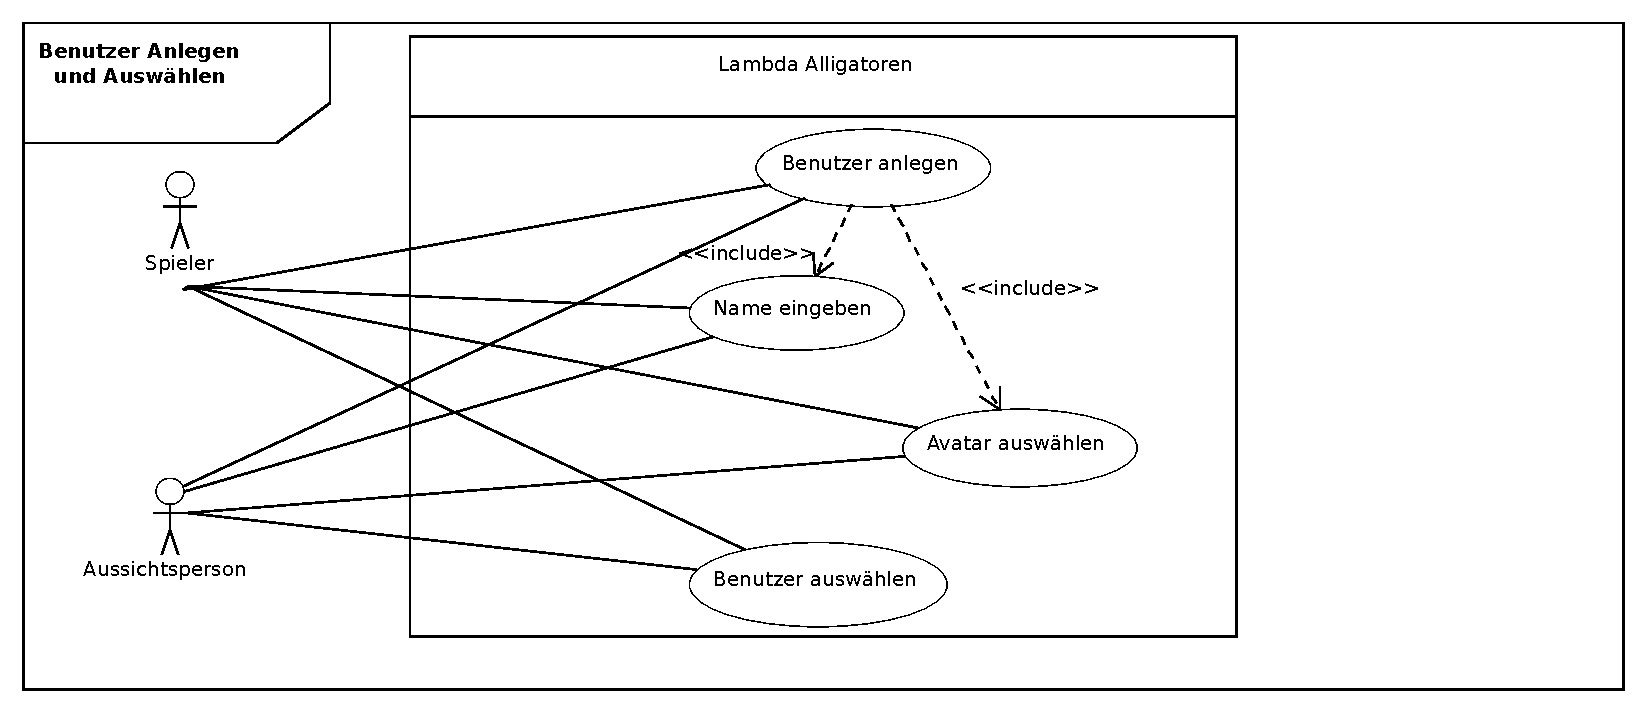
\includegraphics[scale=0.6]{Systemmodelle/add_use_case.pdf}
\captionof{figure}{Anwendungsfall Benutzer Anlegen}
\end{center}
\begin{center}
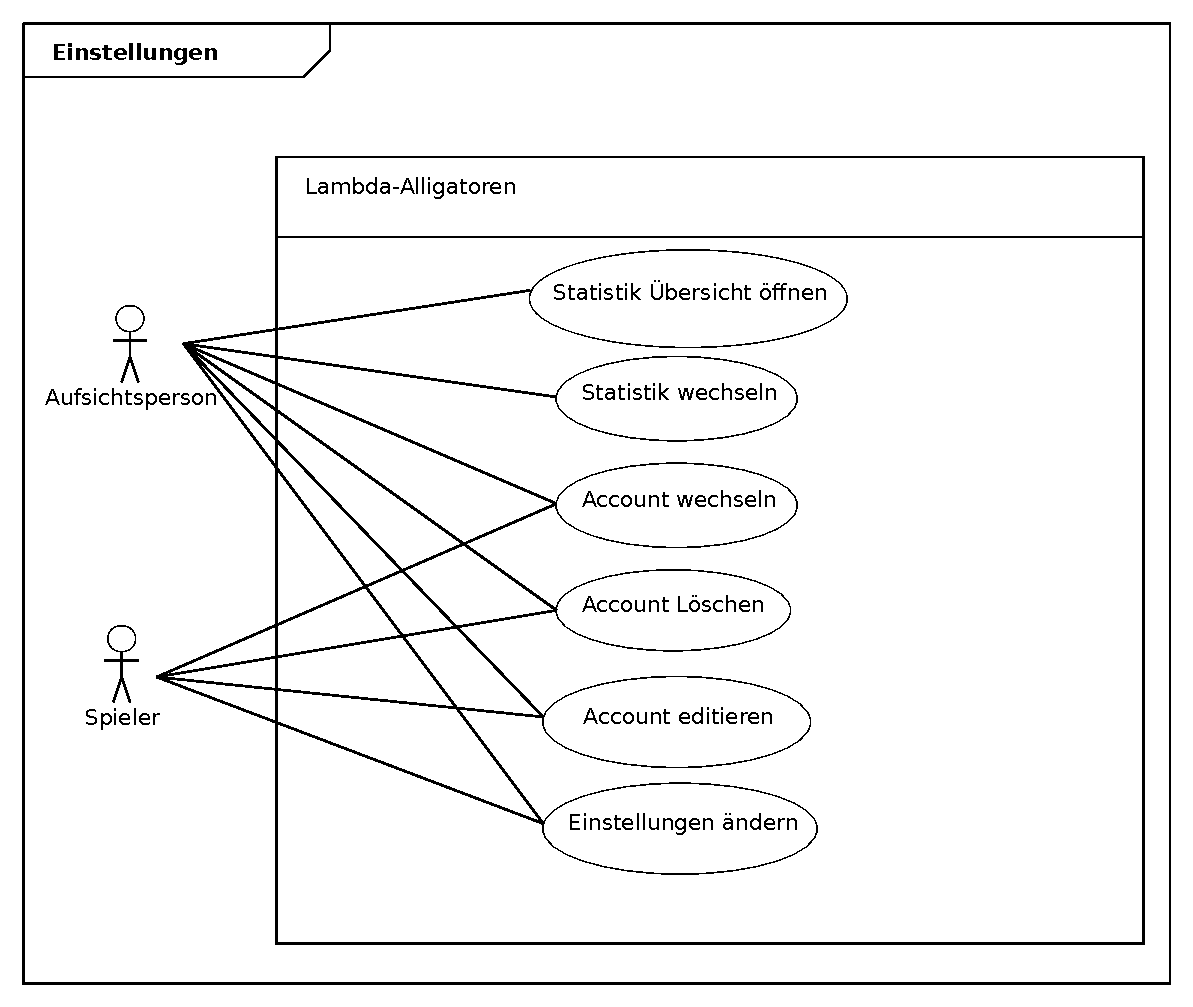
\includegraphics[scale=0.6]{Systemmodelle/settings_use_case.pdf}
\captionof{figure}{Anwendungsfall Einstellungen}
\end{center}
\clearpage
\begin{center}
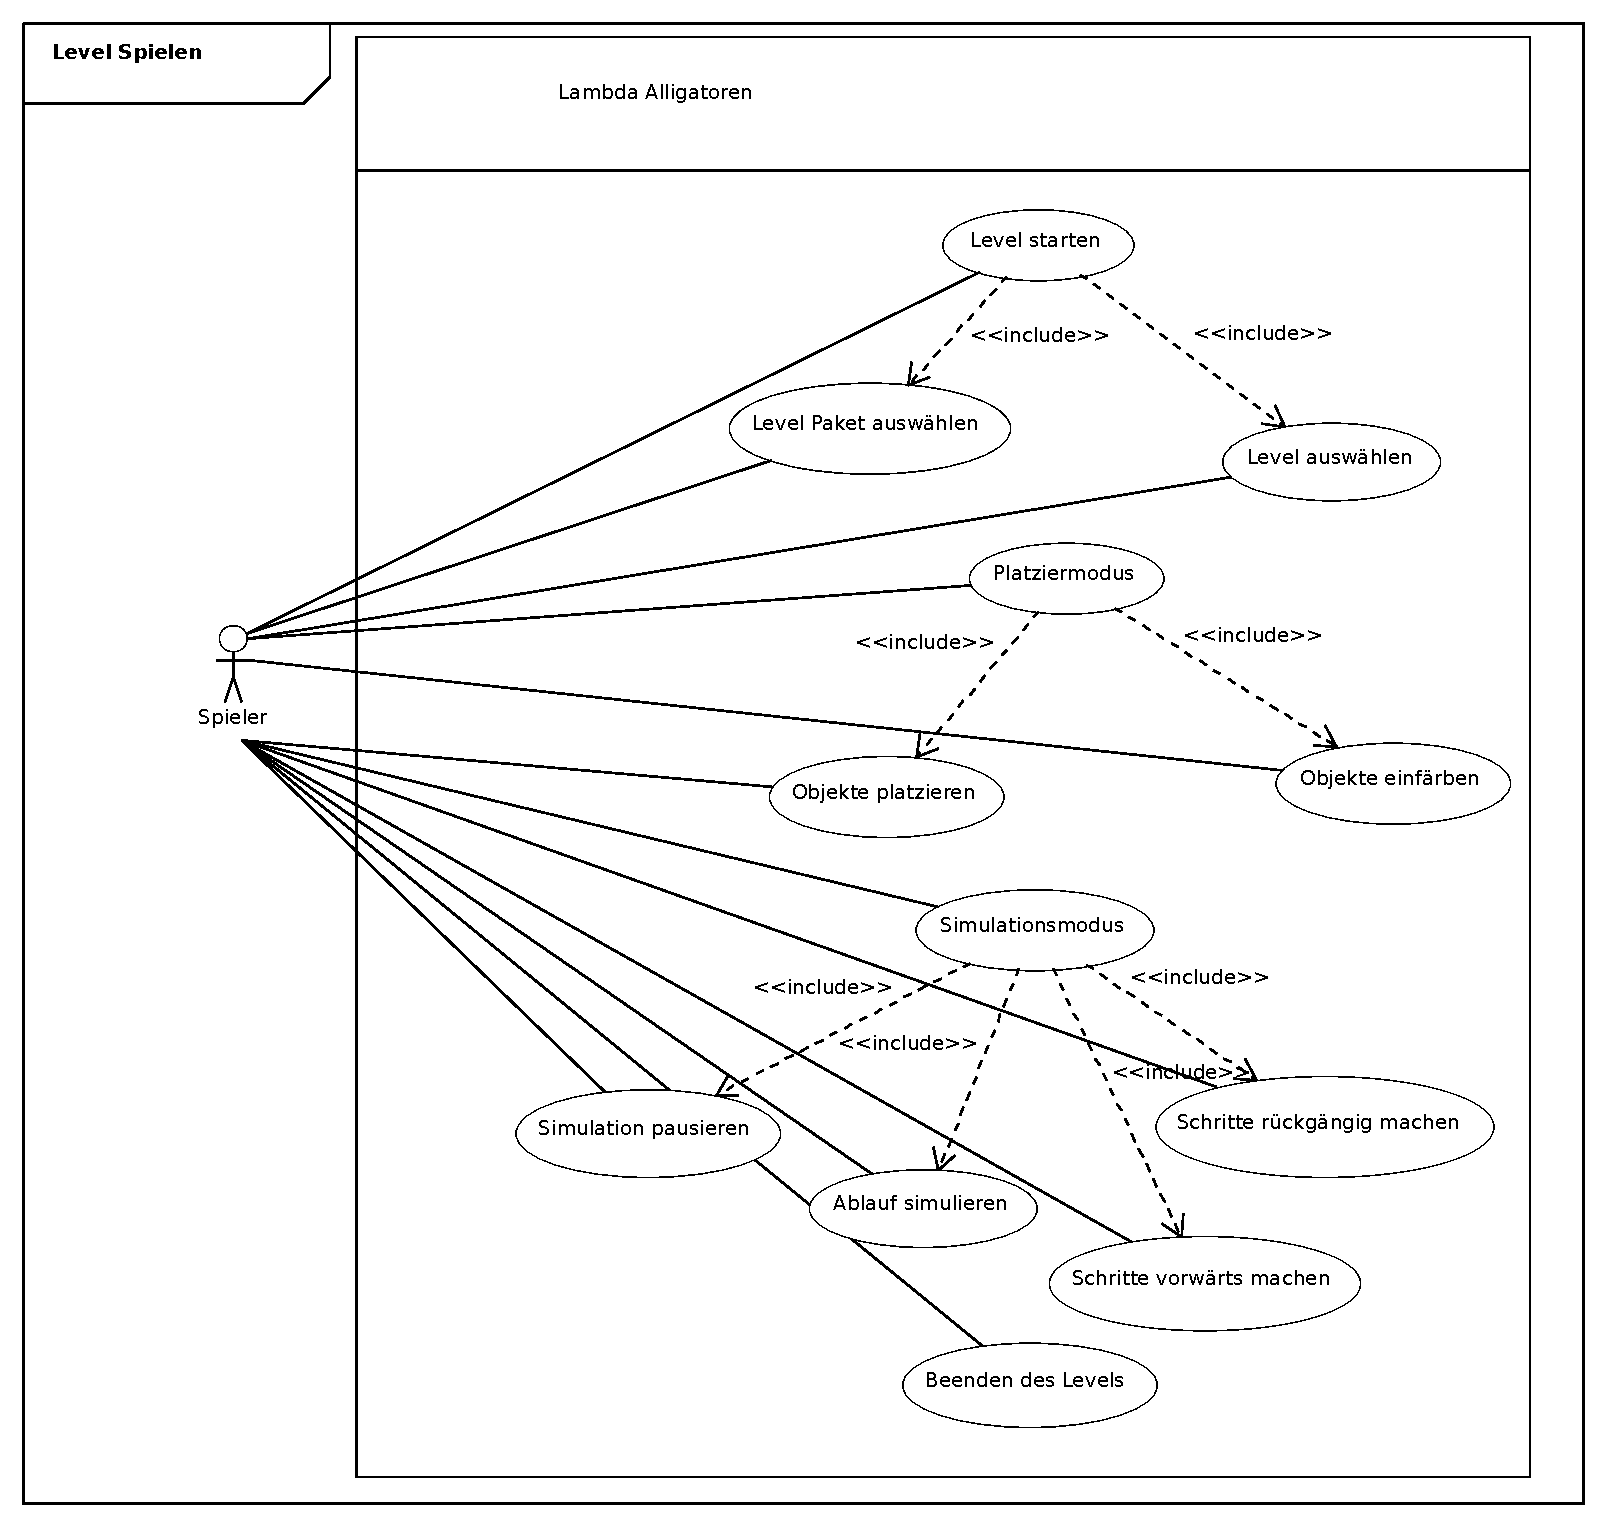
\includegraphics[scale=0.6]{Systemmodelle/level_use_case.pdf}
\captionof{figure}{Anwendungsfall Level Spielen}
\end{center}

\subsection{Objektmodell}
%\clearpage
\begin{center}
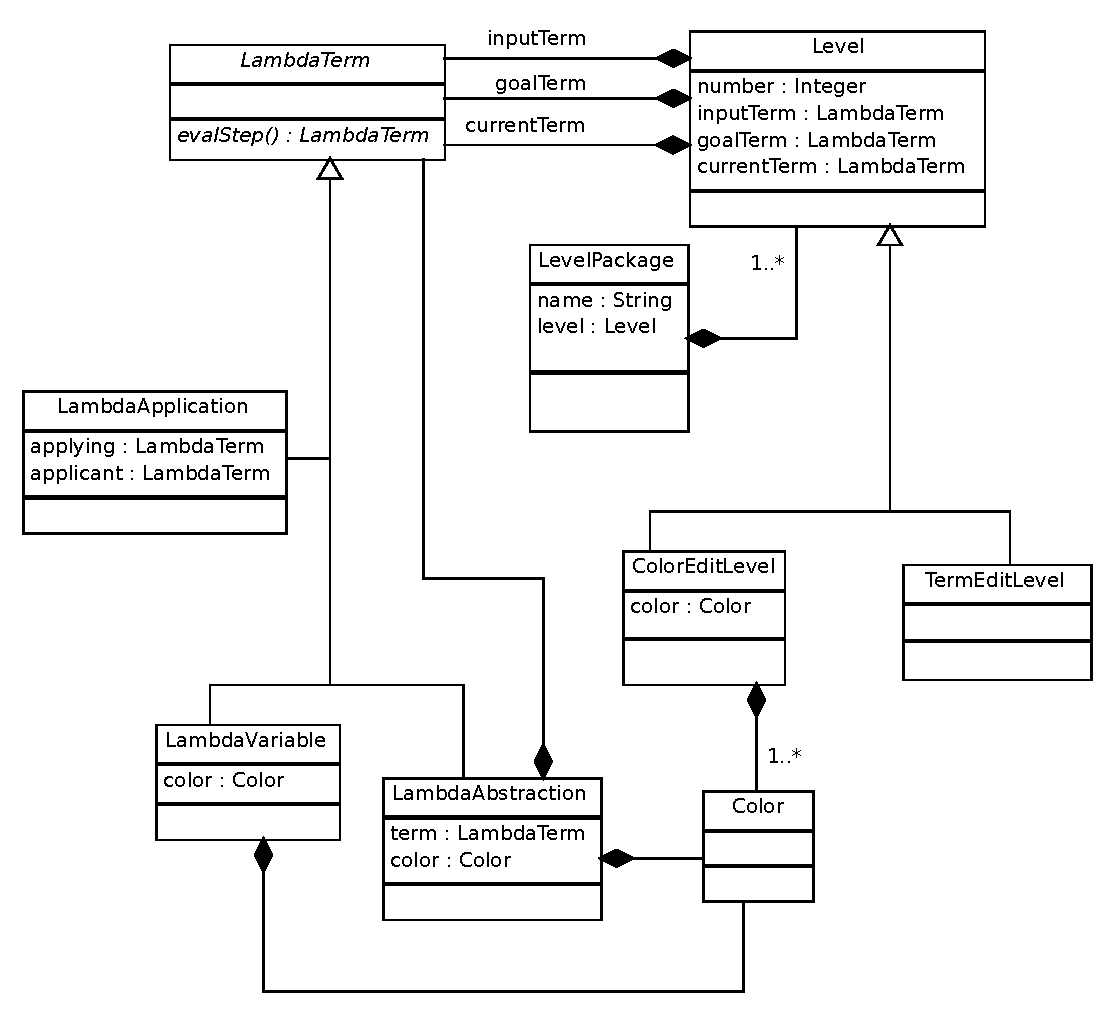
\includegraphics[scale=0.6]{Systemmodelle/level_class.pdf}
\captionof{figure}{Klassendiagramm Level}
\end{center}
\clearpage
\begin{center}
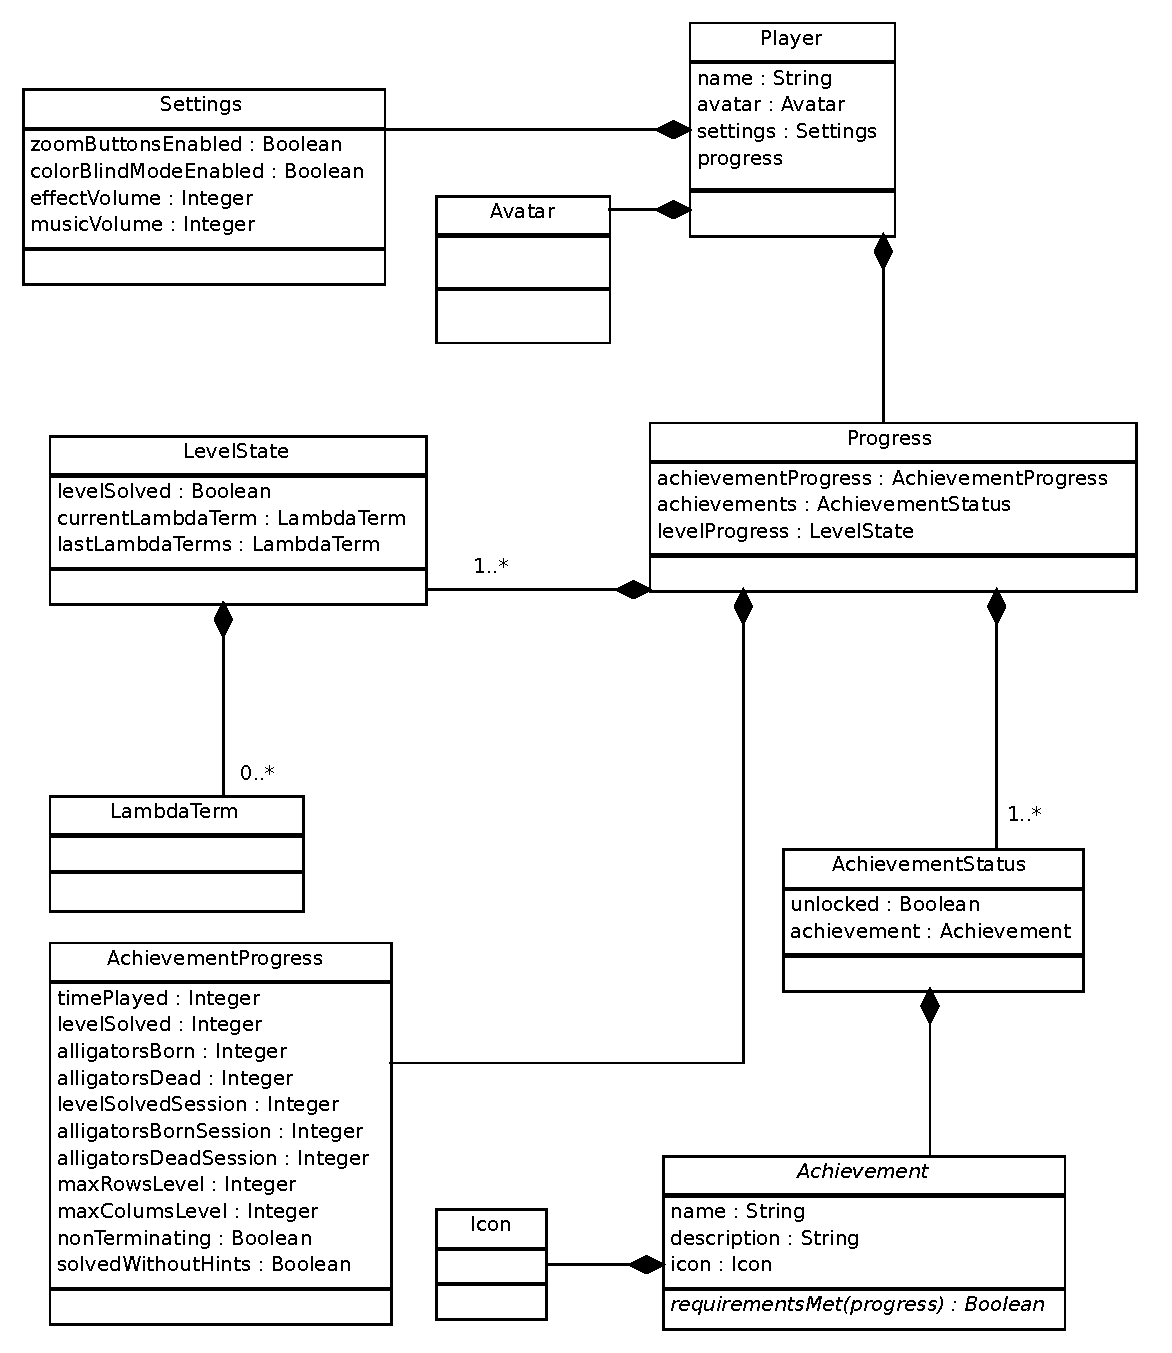
\includegraphics[scale=0.6]{Systemmodelle/player_class.pdf}
\captionof{figure}{Klassendiagramm Player}
\end{center}

\subsection{Dynamische Modelle}
%\clearpage
\begin{center}
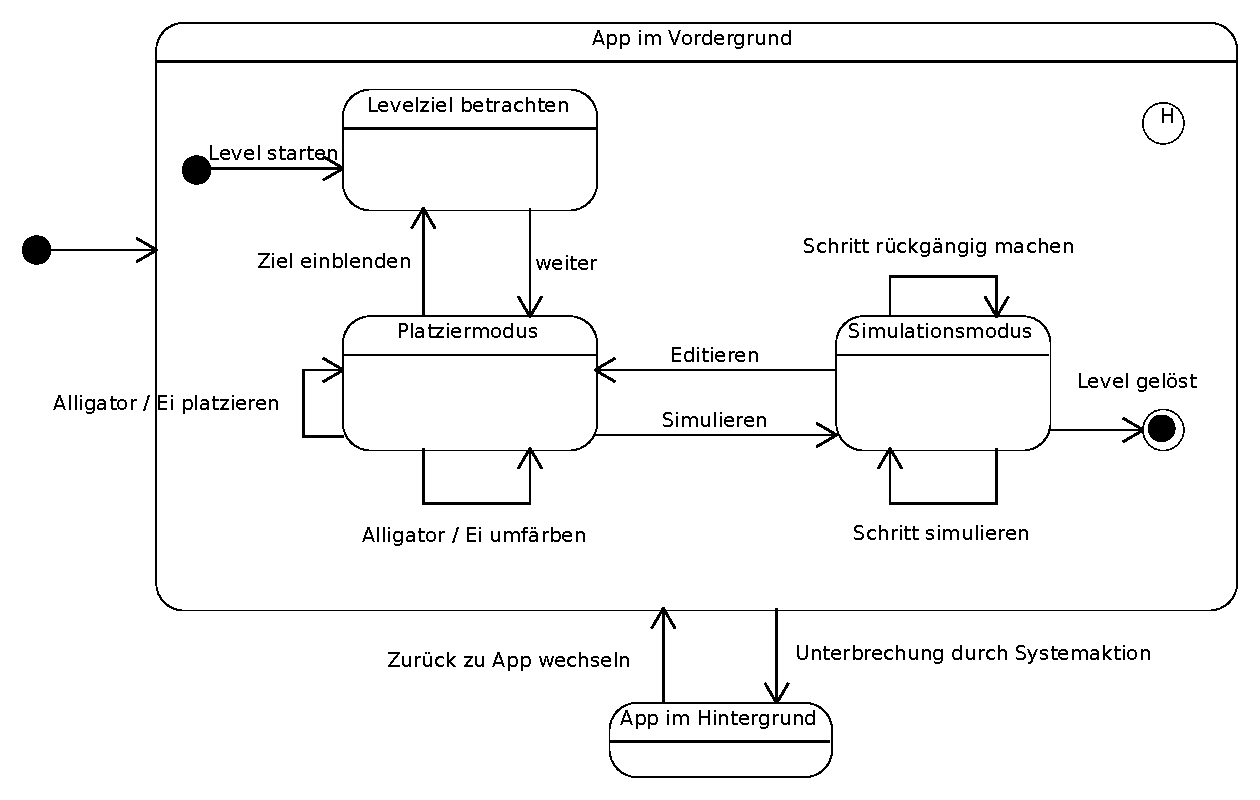
\includegraphics[scale=0.6]{Systemmodelle/game_state.pdf}
\captionof{figure}{Zustandsübergangsdiagramm Spiel}
\end{center}
%\clearpage
%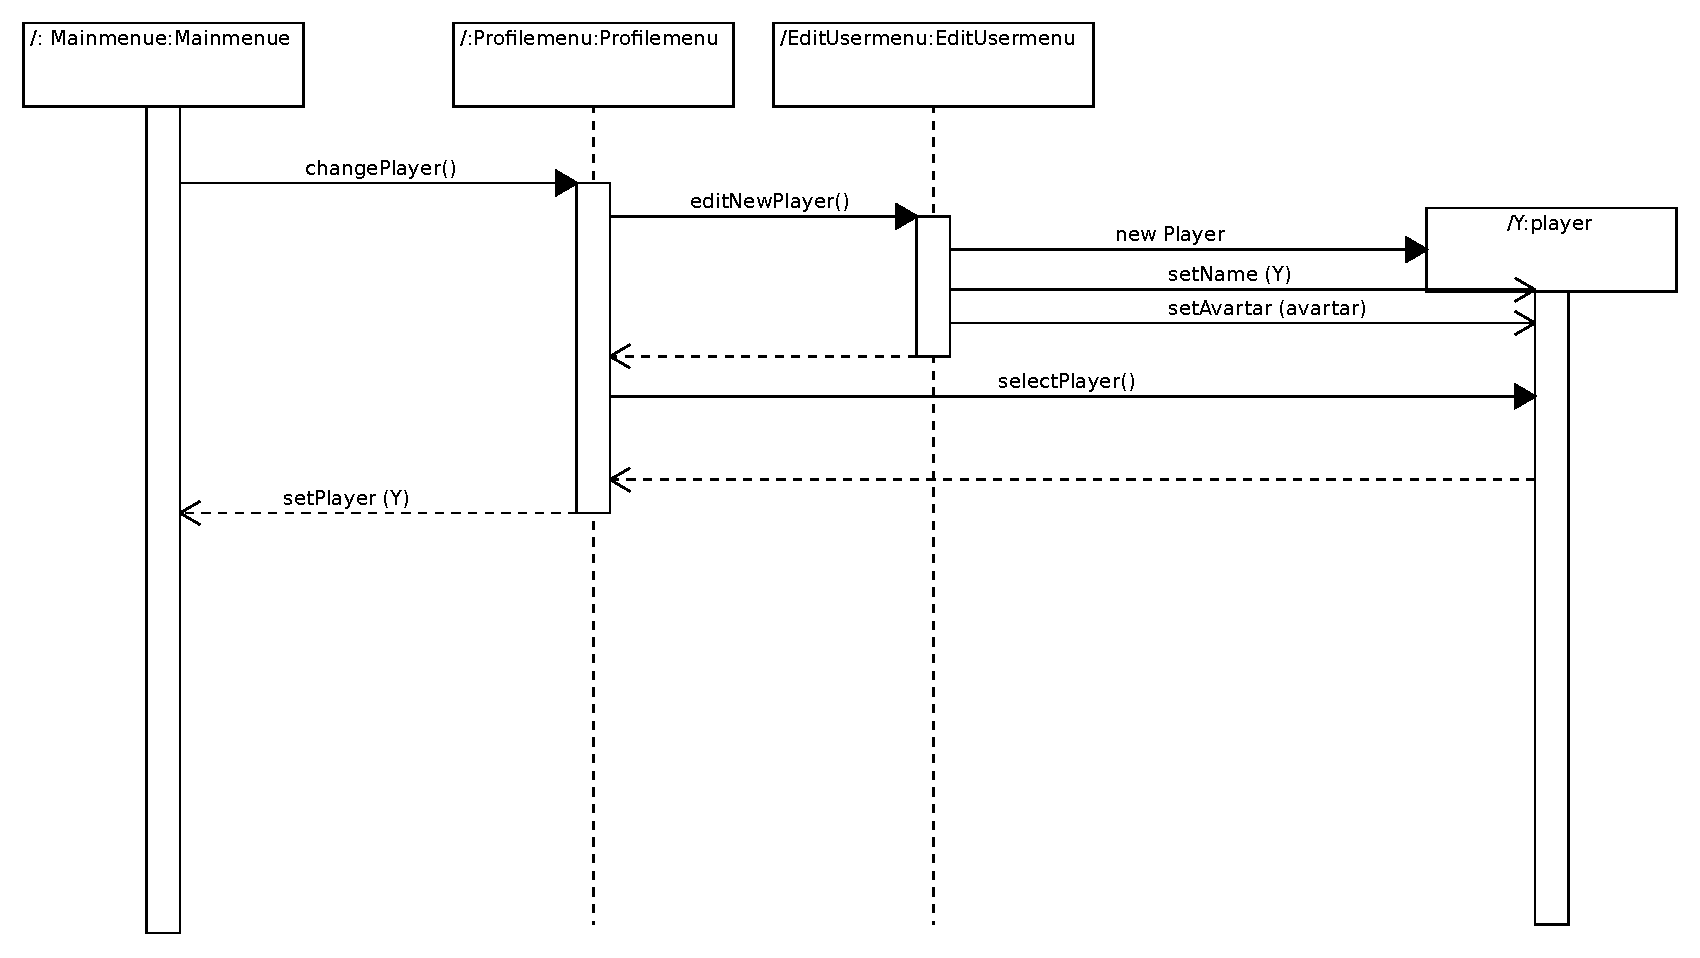
\includegraphics[scale=0.6]{Systemmodelle/edit_new_player_sequence.pdf}
%\clearpage
%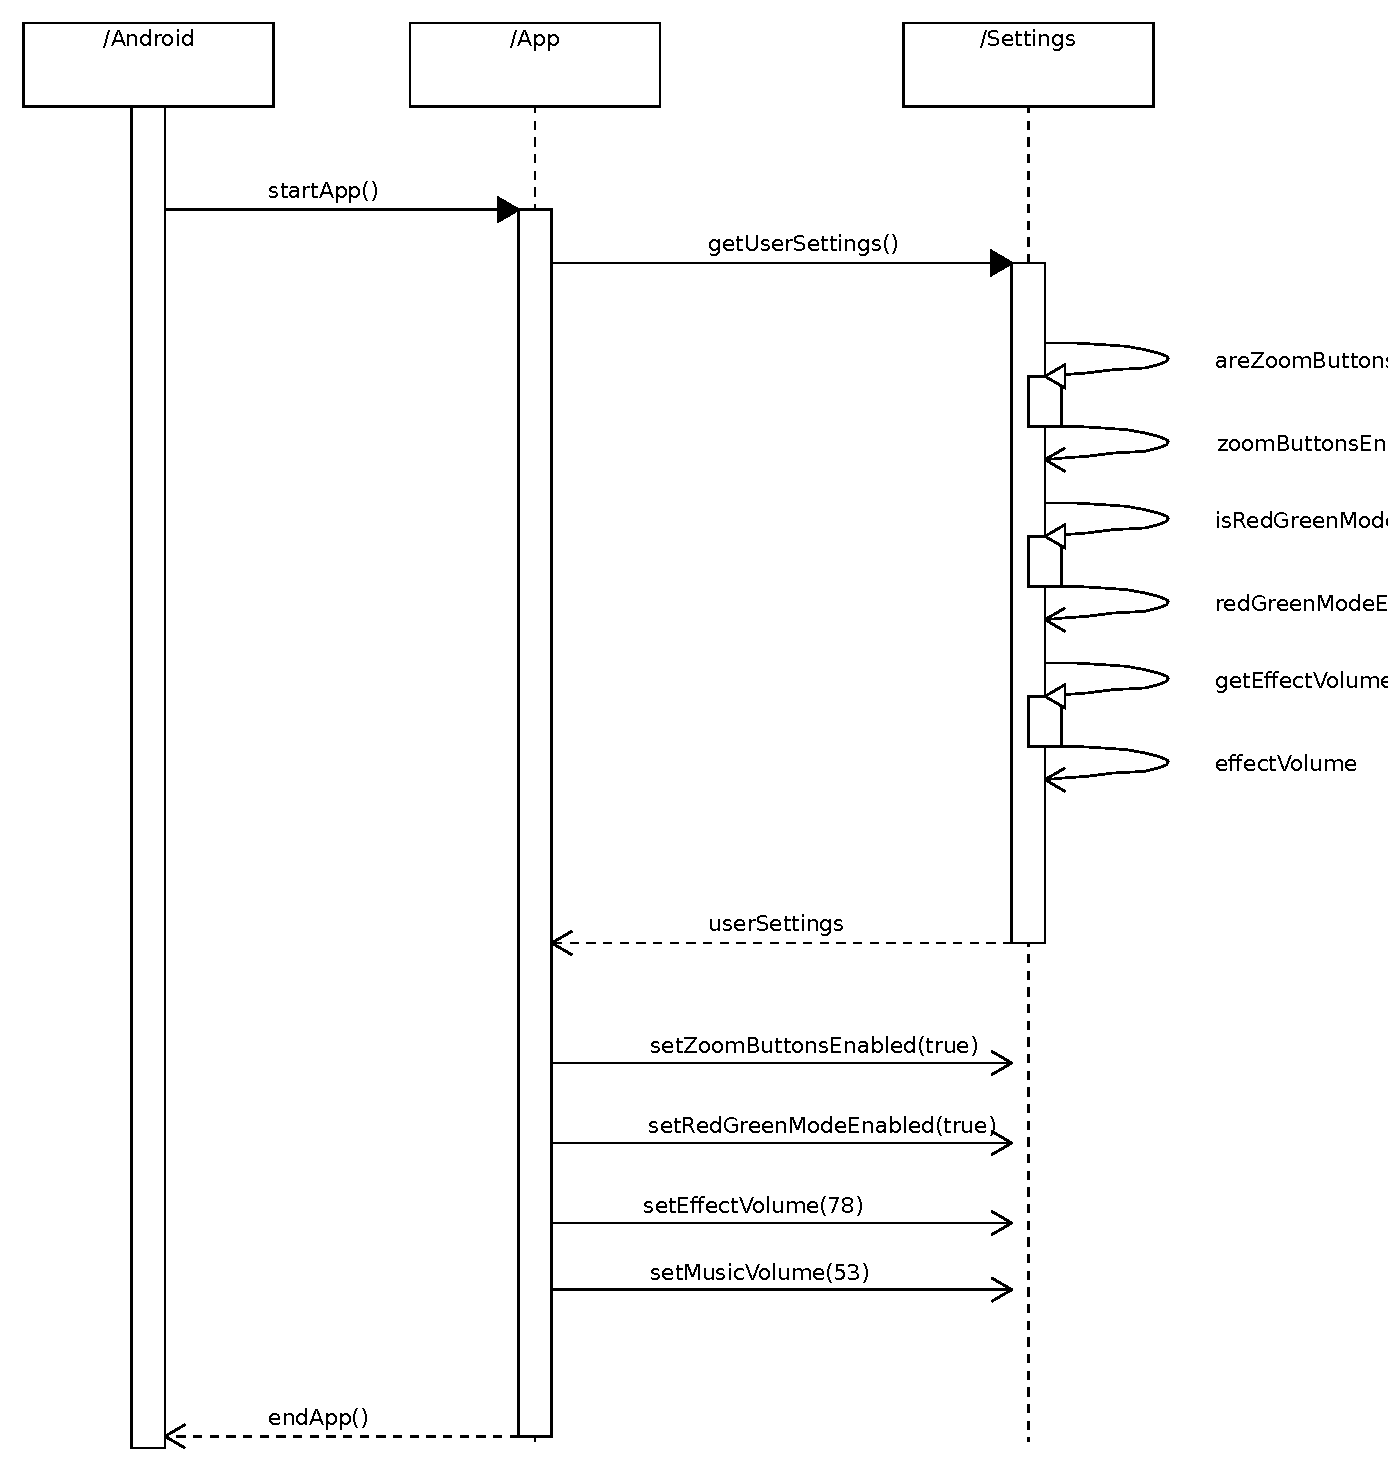
\includegraphics[scale=0.6]{Systemmodelle/edit_settings_sequence.pdf}
%\clearpage
\begin{center}
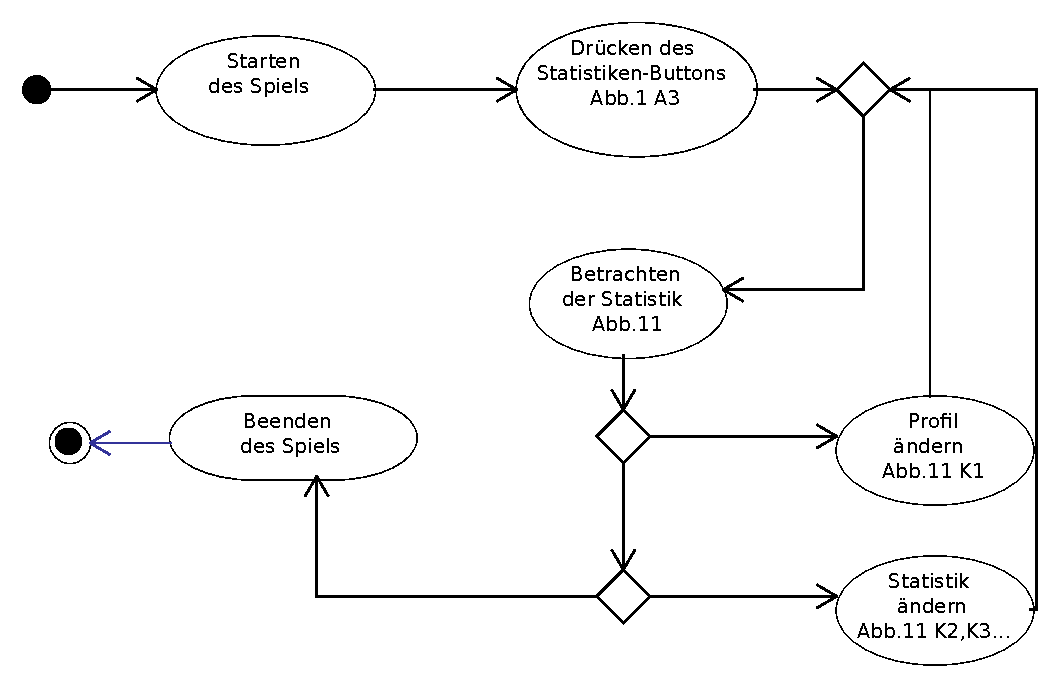
\includegraphics[scale=0.6]{Systemmodelle/parent_activity.pdf}
\captionof{figure}{Aktivitätsdiagramm Elternszenario}
\end{center}
\clearpage
\begin{center}
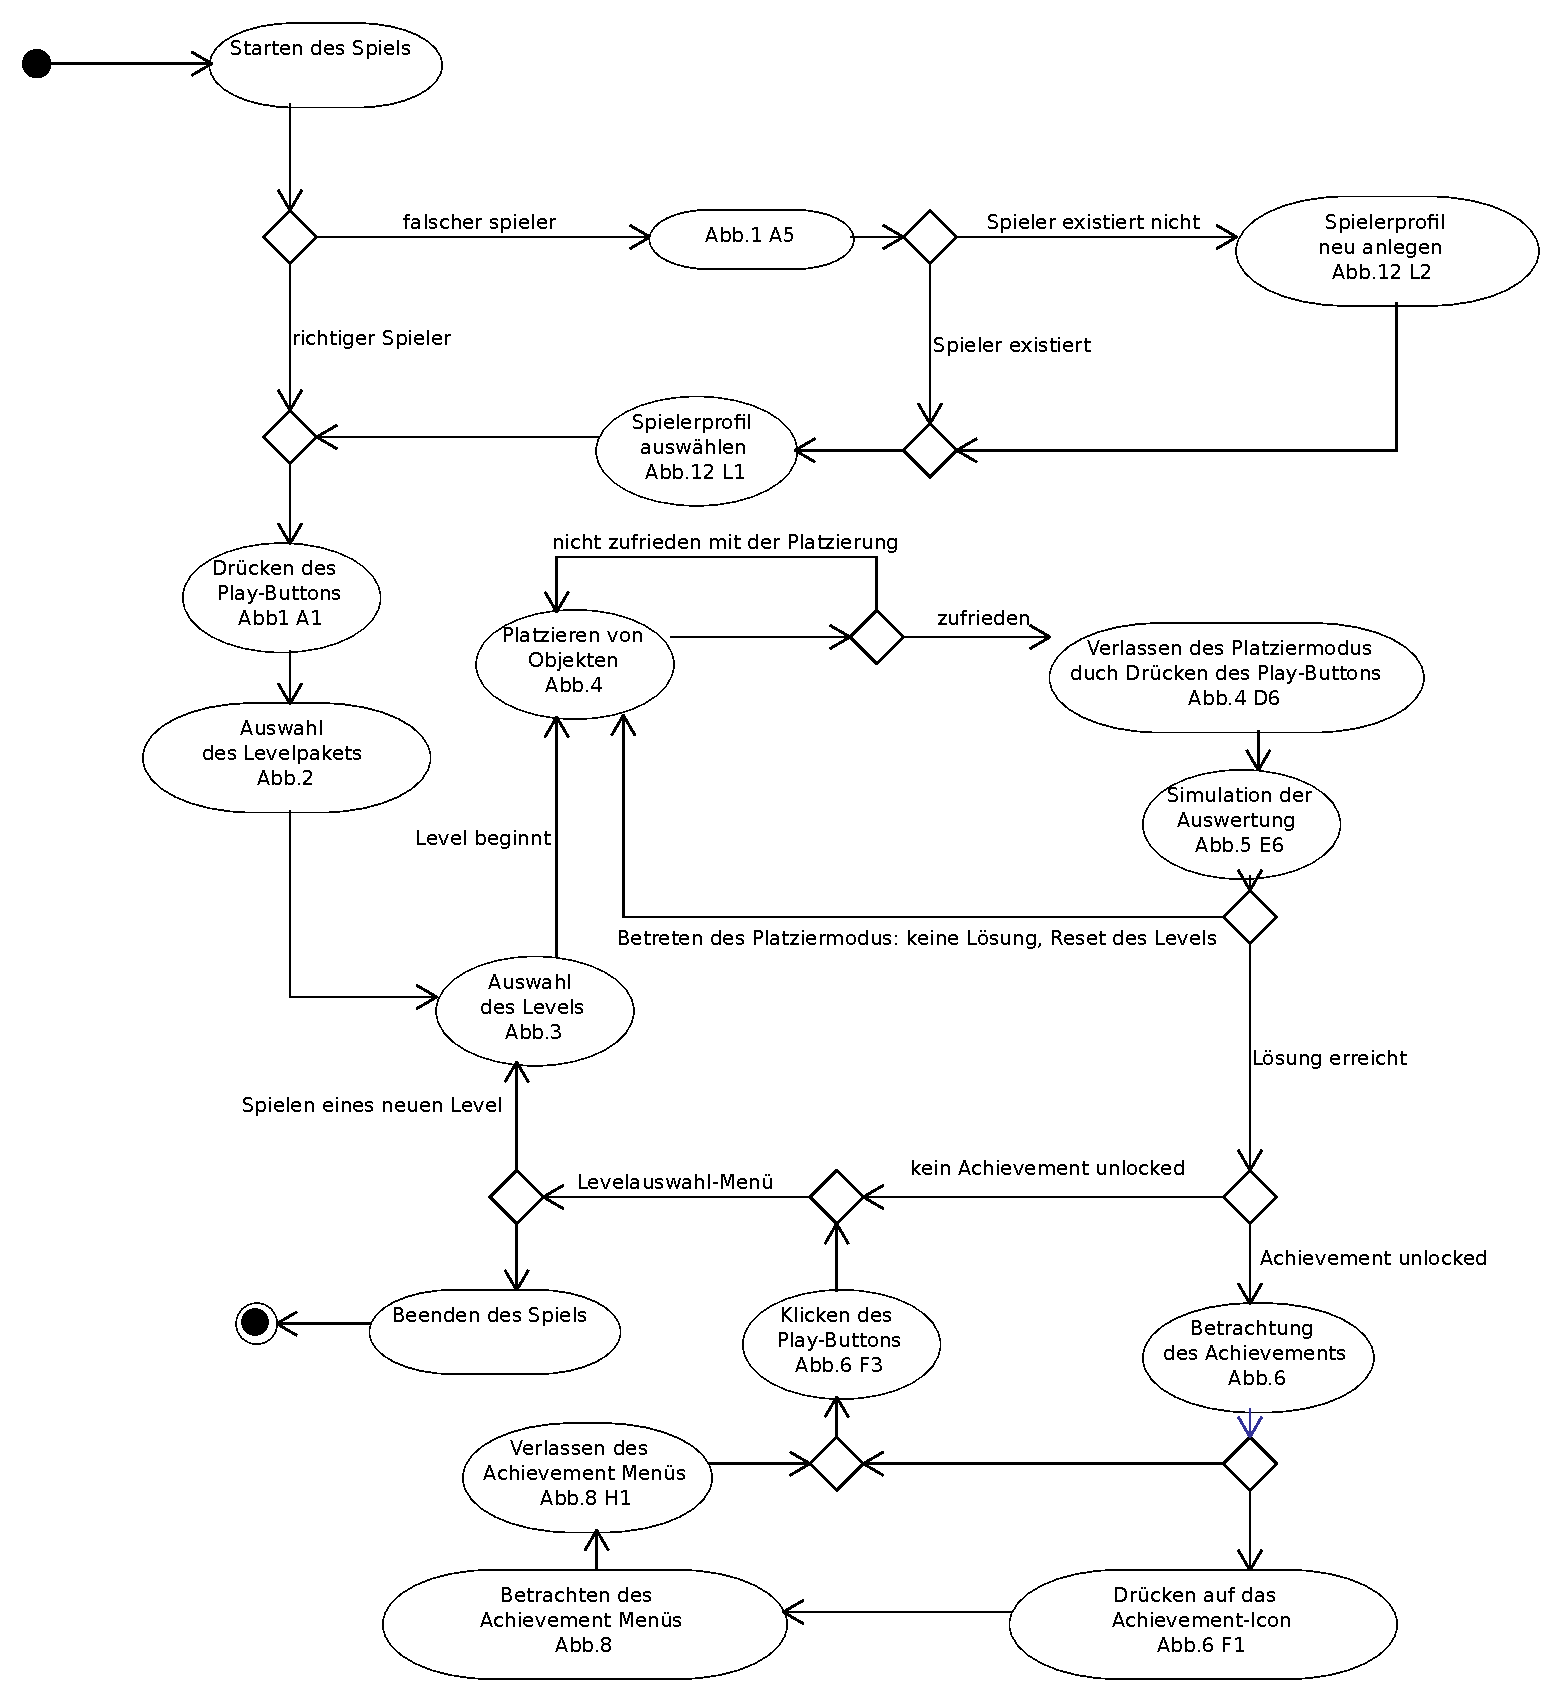
\includegraphics[scale=0.6]{Systemmodelle/start_activity.pdf}
\captionof{figure}{Aktivitätsdiagramm Kind}
\end{center}

\subsection{Benutzerschnittstelle}

\subsubsection{Hauptmenü}

\begin{center}
\setlength\fboxsep{20pt}
\setlength\fboxrule{1pt}
\fbox{
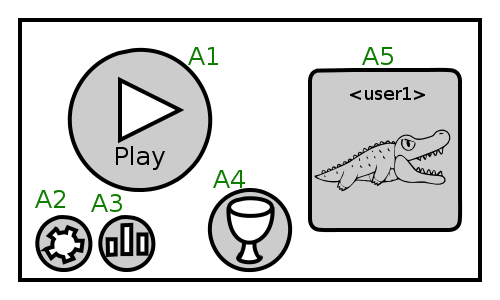
\includegraphics[scale=0.5]{Systemmodelle/images/main_menu.png}
}
\captionof{figure}{Hauptmenü}
\end{center}

Das Hauptmenü wird beim Neustarten der App als Erstes geöffnet. Wird die App zum ersten Mal verwendet oder existieren keine Profile, wird zunächst die Profilerstellung (Teil 1) geöffnet.
\begin{requirements}
\req{A1} Öffnet die Levelübersicht.
\req{A2} Öffnet das Einstellungsmenü.
\req{A3} Öffnet die Statistiken und übernimmt den aktuellen Benutzer als ausgewählten Benutzer in der Statistik.
\req{A4+} Öffnet die Achievements.
\req{A5+} Öffnet die Profilauswahl.
\end{requirements}

\subsubsection{Levelübersicht}

\begin{center}
\setlength\fboxsep{20pt}
\setlength\fboxrule{1pt}
\fbox{
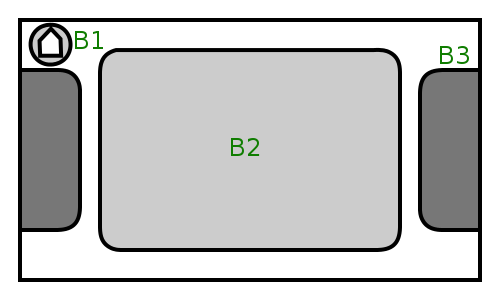
\includegraphics[scale=0.5]{Systemmodelle/images/level_overview.png}
}
\captionof{figure}{Levelübersicht}
\end{center}

\begin{requirements}
\req{B1} Navigiert zurück zum Hauptmenü.
\req{B2} Ein Levelblock repräsentiert eine bestimmte Anzahl und/oder Kategorie von elementaren Leveln. Der Sandbox-Modus wird durch einen Levelblock repräsentiert[+]. Öffnet die Leveldetailübersicht.
\req{B3} Der in der Levelanordnung nächste Levelblock. Wird durch eine Swipe-Geste zentriert und nimmt so den Platz des aktuellen Levelblocks ein.
\end{requirements}

\subsubsection{Leveldetailübersicht}

\begin{center}
\setlength\fboxsep{20pt}
\setlength\fboxrule{1pt}
\fbox{
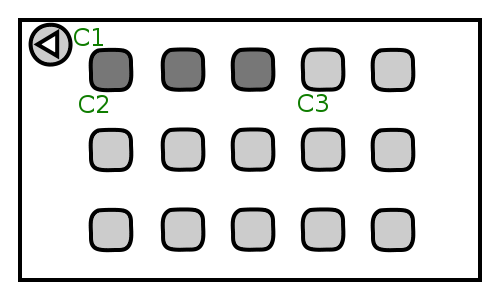
\includegraphics[scale=0.5]{Systemmodelle/images/level_overview_detail.png}
}
\captionof{figure}{Leveldetailübersicht}
\end{center}

\begin{requirements}
\req{C1} Navigiert zurück zur Levelübersicht.
\req{C2} Ein verfügbares Level. Drücken startet das jeweilige Level.
\req{C3} Ein nicht verfügbares Level. Kann durch erfolgreiches Lösen der vorhergehenden Level freigeschaltet werden und wird dann verfügbar.
\end{requirements}

\subsubsection{Level (Platziermodus)}

\begin{center}
\setlength\fboxsep{20pt}
\setlength\fboxrule{1pt}
\fbox{
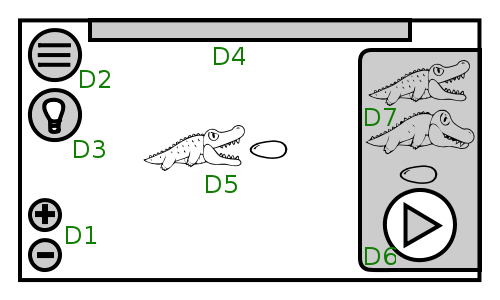
\includegraphics[scale=0.5]{Systemmodelle/images/level.png}
}
\captionof{figure}{Level (Platziermodus)}
\end{center}


\begin{center}
\setlength\fboxsep{20pt}
\setlength\fboxrule{1pt}
\fbox{
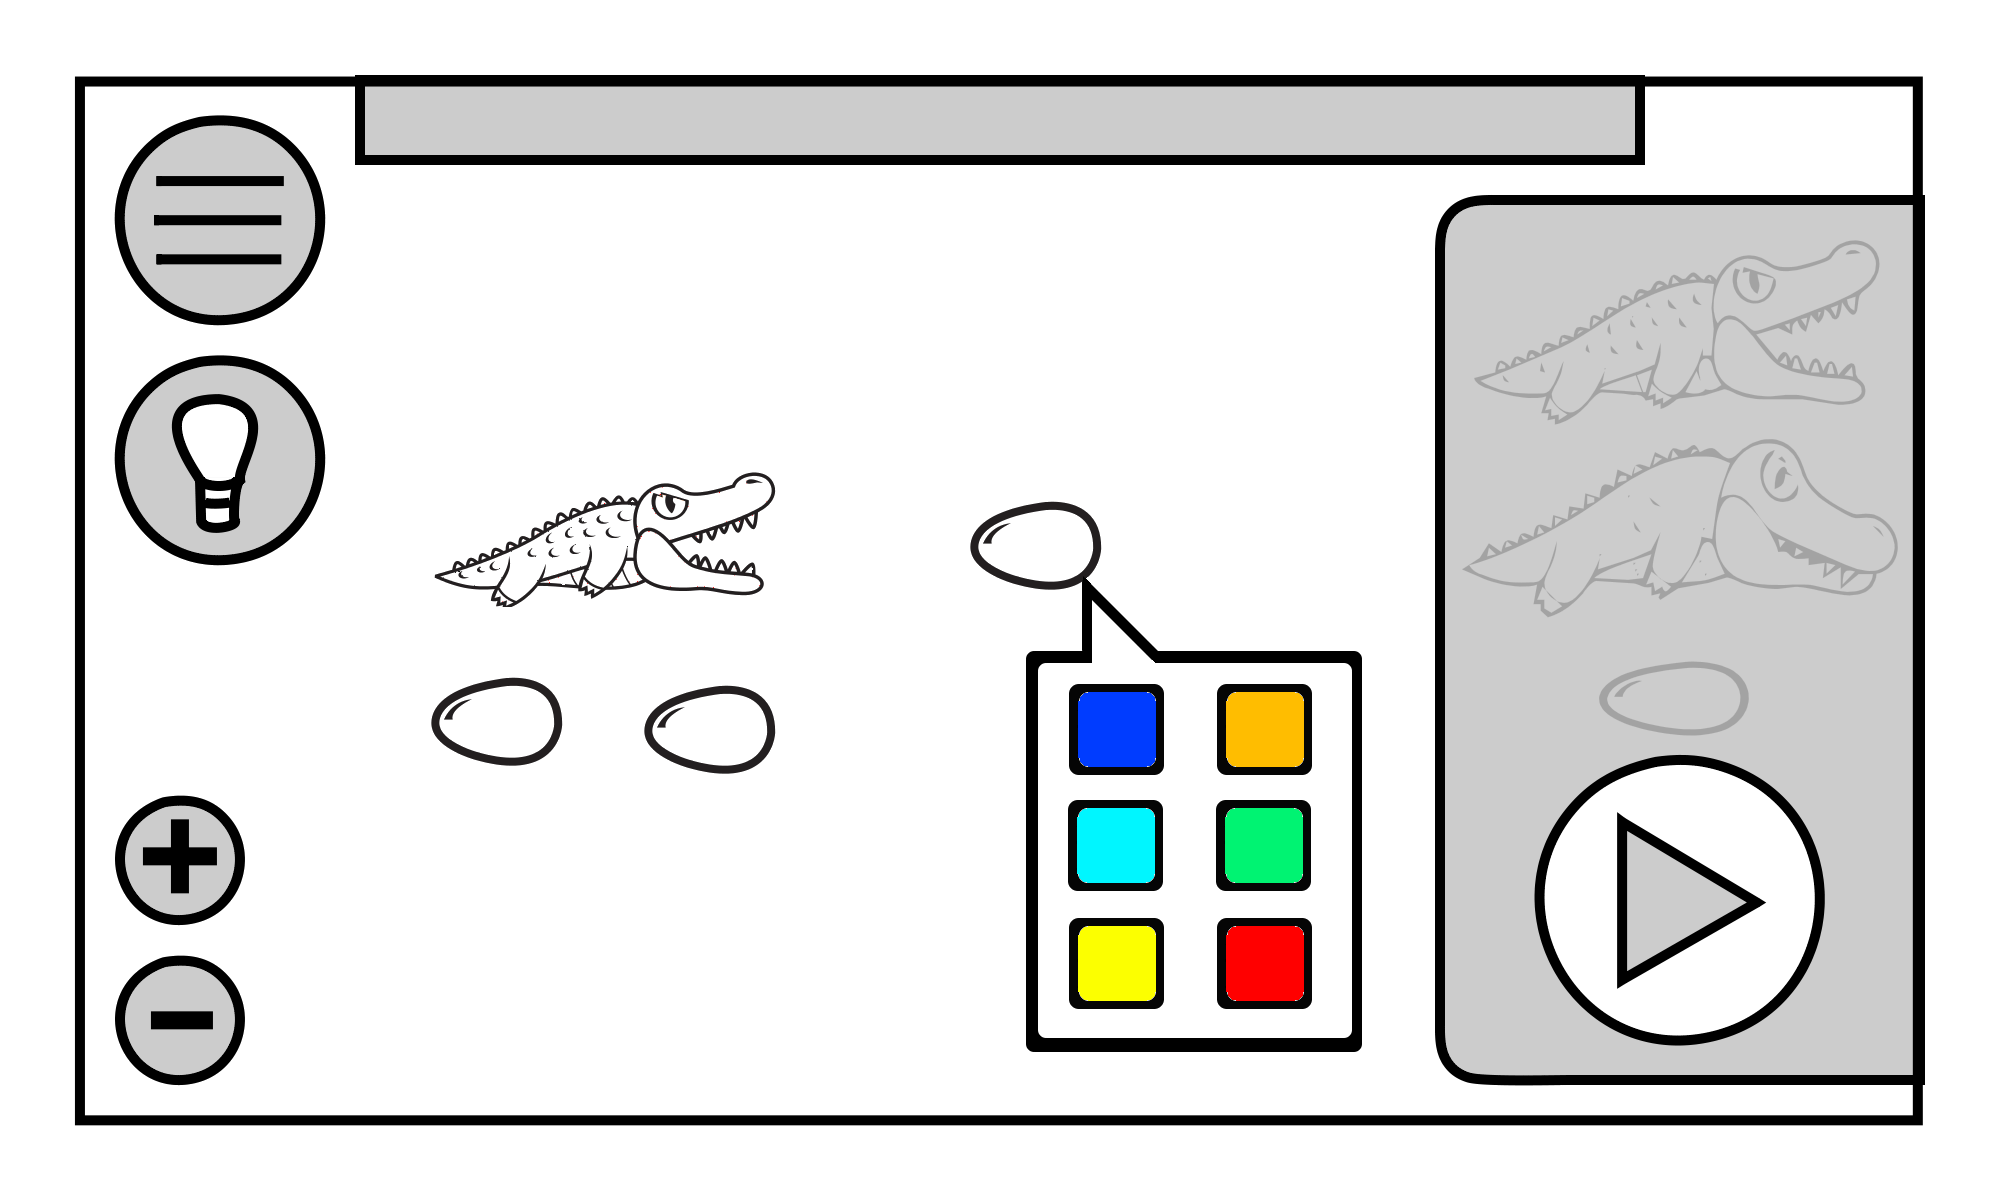
\includegraphics[scale=0.125]{Systemmodelle/images_blank/level_color.png}
}
\captionof{figure}{Farbauswahl}
\label{farbauswahl}
\end{center}


\begin{requirements}
\req{D1} Zoom: Vergrößert/verkleinert die Termansicht. Kann im Einstellungsmenü deaktiviert bzw. aktiviert werden.
\req{D2} Öffnet das Spielmenü.
\req{D3+} Öffnet einen Tipp zur Lösung des Levels. Wird erst nach einer gewissen Zeit, in der das Level nicht gelöst werden konnte, aktiviert.
\req{D4} Anwählen oder nach unten Ziehen zeigt die nach der Auswertung zu erreichende Konstellation an.
\req{D5} Auf der Arbeitsfläche können zu den bereits vom Level vorgegebenen Alligatoren weitere hinzugefügt werden. Anwählen von platzierten Alligatoren öffnet eine Farbübersicht, aus der eine Farbe für diesen Alligator ausgewählt werden kann (vgl. Abb. \ref{farbauswahl})
\req{D6} Startet den Simulationsmodus.
\req{D7} Alligatoren/Eier, welche per Drag\&Drop auf der Arbeitsfläche platziert werden können.
\end{requirements}

\subsubsection{Level (Simulationsmodus)}

\begin{center}
\setlength\fboxsep{20pt}
\setlength\fboxrule{1pt}
\fbox{
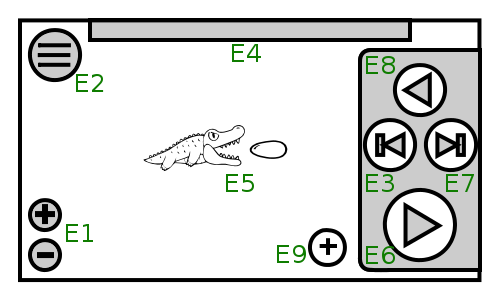
\includegraphics[scale=0.5]{Systemmodelle/images/level_simulation.png}
}
\captionof{figure}{Level (Simulationsmodus)}
\end{center}

\begin{requirements}
\req{E1} Zoom: Vergrößert/verkleinert die Termansicht. Kann im Einstellungsmenü deaktiviert bzw. aktiviert werden.
\req{E2} Öffnet das Spielmenü.
\req{E3+} Setzt, sofern möglich, die Simulation um einen Schritt zurück.
\req{E4} Anwählen oder nach unten Ziehen zeigt die zur Lösung des Levels zu erreichende Konstellation.
\req{E5} Im Simulationsmodus kann die Arbeitsfläche nicht mehr verändert werden.
\req{E6} Startet/pausiert den automatischen Simulationsdurchlauf.
\req{E7} Führt einen einzelnen Schritt der Simulaton aus.
\req{E8} Bricht die Simulation ab und kehrt zum Platziermodus zurück.
\req{E9+} Einstellungsmöglichkeit für die Geschwindigkeit der automatischen Simulation. Es stehen zwei Geschwindigkeitsstufen zur Verfügung.
\end{requirements}

\subsubsection{Levelerfolg}

\begin{center}
\setlength\fboxsep{20pt}
\setlength\fboxrule{1pt}
\fbox{
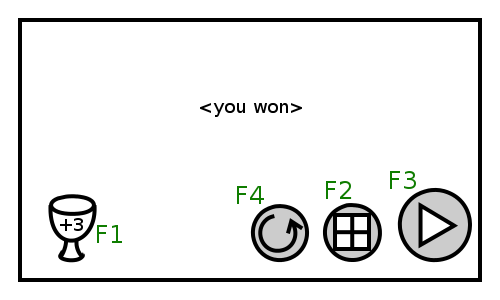
\includegraphics[scale=0.5]{Systemmodelle/images/level_solved.png}
}
\captionof{figure}{Levelerfolg}
\end{center}

Erscheint, sobald im Simulationsmodus die vorgegebene Endkonstellation oder die erforderliche Anzahl an Auswertungsschritten erreicht wurde.
\begin{requirements}
\req{F1+} Stellt die Anzahl der im Level freigeschalteten Achievements dar.
\req{F2} Navigiert zur Levelübersicht.
\req{F3} Startet sofern möglich automatisch das nächste Level, .
\req{F4} Startet das aktuelle Level erneut.
\end{requirements}

\subsubsection{Spielmenü}

\begin{center}
\setlength\fboxsep{20pt}
\setlength\fboxrule{1pt}
\fbox{
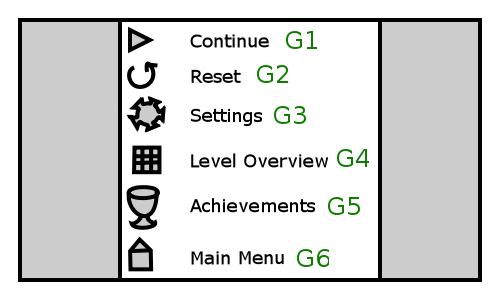
\includegraphics[scale=0.5]{Systemmodelle/images/ingame_menu.png}
}
\captionof{figure}{Spielmenü}
\end{center}

\begin{requirements}
\req{G1} Wechselt zurück zum laufenden Level.
\req{G2} Verwirft den aktuellen Zustand des Levels und setzt es zurück.
\req{G3} Öffnet das Einstellungsmenü.
\req{G4} Navigiert zurück zur Leveldetailübersicht.
\req{G5+} Öffnet die Achievements.
\req{G6} Navigiert zurück zum Hauptmenü.
\end{requirements}

\subsubsection{Achievements}

\begin{center}
\setlength\fboxsep{20pt}
\setlength\fboxrule{1pt}
\fbox{
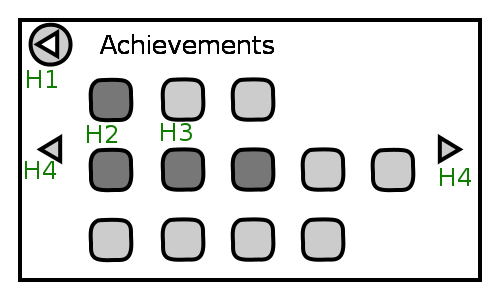
\includegraphics[scale=0.5]{Systemmodelle/images/achievements.png}
}
\captionof{figure}{Achievements}
\end{center}

\begin{requirements}
\req{H1+} Navigiert zurück zum vorherigen Navigationpunkt (Spielmenü oder Hauptmenü).
\req{H2+} Erreichtes Achievement. Öffnet die Detailansicht mit Icon und Beschreibung des angewählten Achievements.
\req{H3+} Noch nicht erreichtes Achievement. Ist wahlweise ausgegraut oder unsichtbar. Öffnet, falls nicht unsichtbar, eine Beschreibung, wie das gewählte Achievement zu erreichen ist.
\req{H4+} Navigiert zum vorigen/nächsten Achievementblock.
\end{requirements}

\subsubsection{Achievement-Benachrichtigung}

\begin{center}
\setlength\fboxsep{20pt}
\setlength\fboxrule{1pt}
\fbox{
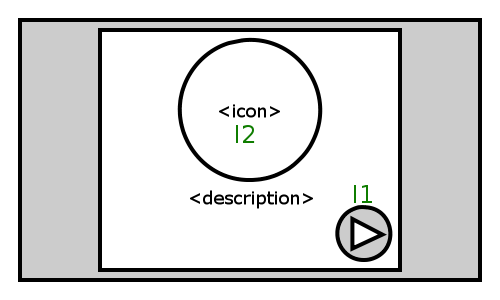
\includegraphics[scale=0.5]{Systemmodelle/images/achievement_notification.png}
}
\captionof{figure}{Achievement-Benachrichtigung}
\end{center}

Alle Achievement-Benachrichtigungen werden nach erfolgreichem Abschluss eines Levels angezeigt.
\begin{requirements}
\req{I1+} Schließt die Benachrichtigung. Wurden weitere Achievements erreicht, erscheint die nächste Benachrichtigung, ansonsten wird mit dem üblichen Levelschema fortgefahren. 
\req{I2+} Icon des Achievements durch drücken öffnet sich die Achievements.
\end{requirements} 

\subsubsection{Einstellungsmenü}

\begin{center}
\setlength\fboxsep{20pt}
\setlength\fboxrule{1pt}
\fbox{
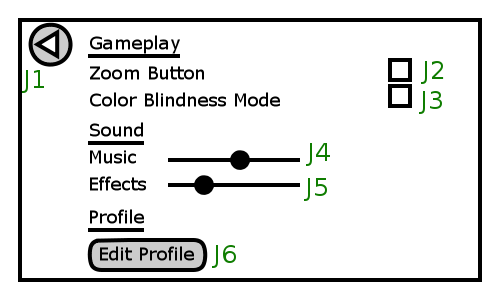
\includegraphics[scale=0.5]{Systemmodelle/images/settings.png}
}
\captionof{figure}{Einstellungsmenü}
\end{center}

\begin{requirements}
\req{J1} Navigiert zurück zum vorherigen Navigationpunkt (Spielmenü oder Hauptmenü).
\req{J2} (De-)Aktiviert die buttongesteuerte Zoomfunktion im Level (statt dem üblichen Multitouch-Zoom).
\req{J3+} (De-)Aktiviert den Farbenblindheitsmodus.
\req{J4+} Setzt die Musiklautstärke.
\req{J5+} Setzt die Effektlautstärke.
\req{J6+} Öffnet ein Menü mit den Optionen zum Bearbeiten des Profils (Name ändern/Profilbild ändern/Löschen).
\end{requirements}

\subsubsection{Statistiken}

\begin{center}
\setlength\fboxsep{20pt}
\setlength\fboxrule{1pt}
\fbox{
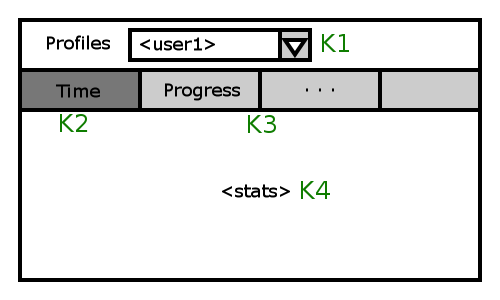
\includegraphics[scale=0.5]{Systemmodelle/images/stats.png}
}
\captionof{figure}{Statistiken}
\end{center}

\begin{requirements}
\req{K1+} Aktuell ausgewählter Benutzer. Beim Öffnen der Statistiken ist der Benutzer ausgewählt, von dessen Profil aus die Statistiken geöffnet wurden. Öffnet ein Dropdownmenü zur Auswahl eines Benutzers.
\req{K2} Aktuell ausgewählter Tab.
\req{K3} Restliche thematische Tabs. Können durch Drücken gewählt oder durch Swipe-Navigation erreicht werden. Tableiste kann je nach Anzahl der Tabs gescrollt werden.
\req{K4} Statistikeinträge sind durch Tableiste thematisch gruppiert und können je nach Anzahl der Einträge gescrollt werden.
\end{requirements}

\subsubsection{Profilauswahl}

\begin{center}
\setlength\fboxsep{20pt}
\setlength\fboxrule{1pt}
\fbox{
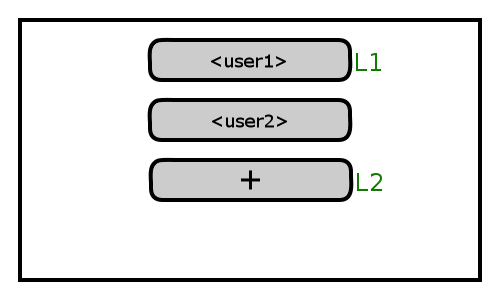
\includegraphics[scale=0.5]{Systemmodelle/images/change_user.png}
}
\captionof{figure}{Profilauswahl}
\end{center}

\begin{requirements}
\req{L1+} Selektiert das gewählte Profil und öffnet dessen Hauptmenü.
\req{L2+} Öffnet den Profilerstellungsdialog.
\end{requirements}

\subsubsection{Profilerstellung(Teil 1)}

\begin{center}
\setlength\fboxsep{20pt}
\setlength\fboxrule{1pt}
\fbox{
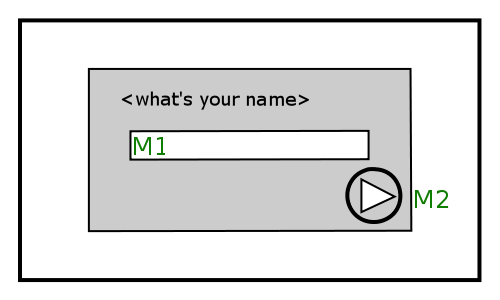
\includegraphics[scale=0.5]{Systemmodelle/images/profile_creator_1.png}
}
\captionof{figure}{Profilerstellung (Teil 1)}
\end{center}

Wird bei erstmaliger Benutzung der App als Erstes geöffnet.
\begin{requirements}
\req{M1} Texteingabefeld für den Benutzernamen. Öffnet die Eingabemethode.
\req{M2+} Bestätigt den eingegebenen Namen und fährt mit Profilerstellung (Teil 2) fort. Falls der eingegebene Name ungültig (z.B. leer) ist oder schon ein Profil mit diesem Benutzernamen existiert, wird eine entsprechende Meldung und eine Möglichkeit zur Änderung der Eingabe gegeben.
\end{requirements}

\subsubsection{Profilerstellung(Teil 2)}

\begin{center}
\setlength\fboxsep{20pt}
\setlength\fboxrule{1pt}
\fbox{
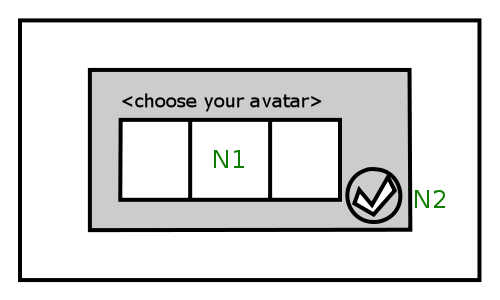
\includegraphics[scale=0.5]{Systemmodelle/images/profile_creator_2.png}
}
\captionof{figure}{Profilerstellung (Teil 2)}
\end{center}

\begin{requirements}
\req{N1+} Wahlmöglichkeiten für das Profilbild. Selektiert und markiert das gewählte Bild. Wird eventuell durch einen umfangreicheren Dialog ersetzt.
\req{N2+} Bestätigt das ausgewählte Bild, erstellt ein Profil und öffnet dessen Hauptmenü.
\end{requirements}



\section{Glossar}
\begin{description}
	\item[Achievement] Deutsch: "`Errungenschaft"'. Zusätzliches Spielziel, das nicht für den eigentlichen Spielverlauf relevant ist, aber zur Motiviation des Spielers dient.
		Der Spieler kann die erlangten Achievements betrachten und bekommt beim Erreichen des Ziels den Erfolg mitgeteilt.
	\item[API-Level] API ist die Abkürzung für Application Programming Interface (deutsch: Schnittstelle zur Anwendungsprogrammierung).
	Das API-Level zeigt die Version der API an, und damit im Falle von Android auch die älteste Androidversion, mit der die Anwendung funktioniert.
	\item[Assets] Medien, also u.A. Soundeffekte, Melodien und Grafiken
	\item[Automatische{[}r{]} Simulation{[}smodus{]}] Funktion, die Schritte innerhalb des Simulationsmodus automatisiert ausführt. Diese kann jederzeit gestartet sowie pausiert werden.
	\item [Avatar bzw. Spieleravatar] Ein Symbol oder eine Figur, die eine bestimmte Person in einem Spiel oder im Internet representiert.
	\item [Drag\&Drop] Deutsch: "`Ziehen und Ablegen"'. Bedienungsart  einer graphischen Benutzeroberfläche durch ein Zeigerelement, dass Elemente ergreift und verschiebt.
	\item [ISCED] International Standard Classification of Education. Ein internationaler Bildungsstandart der UNESCO, um die Schulsysteme verschiedener Länder in einem vergleichbares Format darzustellen.
	\item [Konstellation] Die Representation eines Lambda-Terms durch Alligatoren und Eier auf dem Spielfeld.
	\item[Lambda-Kalkül (\(\lambda\)-Kalkül)] Eine formale Sprache. \url{http://de.wikipedia.org/wiki/Lambda-Kalkül}
	\item[Lambda-Term (\(\lambda\)-Term)] Ein formaler Ausdruck im \(\lambda\)-Kalkül.
		Er kann durch Anwendung der Regeln des Kalküls ausgewertet werden.
	\item[Level] Logischer Spielabschnitt, hier meist eine Rätselaufgabe.
	\item [Piktogramm] Ein einzelnes Symbol, dass seine Information durch vereinfachte graphische Darstellung vermittelt.
	\item [Pinchgeste]auch "`pinch-to-zoom"' Geste genannt: Das Auseinanderspreizen bzw. Zusammenziehen von Daumen und Zeigefinger. Üblicherweise wird sie zum Zoomen genutzt.
	\item [Sandbox] Deutsch: "`Sandkasten"'. Ein Bereich mit minimalen Restriktionen seitens des Spiels und ohne Zielvorgabe.
	\item[Simulationsmodus] Modus, in dem der aktuelle Zustand des Spielfelds schrittweise nach den Regeln des \(\lambda\)-Kalküls ausgewertet wird.
	\item[Smartphone] Ein Mobiltelefon, dass in der Lage ist viele der Funktionen eines Computers auszuführen. Üblicherweise verfügt es über ein großes Display und Touchbedienung.
	\item[Tablet bzw. Tablet Computer] Ein dem Smartphone ähnliches mobiles Endgerät, dass jedoch über eine größere Bildschirmdiagonale verfügt.
	\item[Tutoriallevel] Hinführung und Erklärung zu einer neuen Problemstellung im Spiel. Beispiele können das Verstehen beschleunigen.
	\item[Zoom] Das flüssige Skalieren des gezeigten Spielausschnitts.
\end{description}


\end{document}
